% ---
% Arquivo com a metodologia do Trabalho de Conclusão de Curso dos alunos
% Gabriel Takaoka Nishimura, Felippe Demarqui Ramos e Vivian Kimie Isuyama 
% da Escola Politécnica da Universidade de São Paulo
% ---
	% ---
	\chapter{Metodologia}\label{cap-metodologia}
	% ---
	
	Nesse capítulo são discorridas as escolhas da \texttt{norma 802.15.7}, \textit{hardware} e \texttt{software}.
	
	% ---
	\section{Planejamento}\label{sec-planejamento}
	% ---
	
	% ---
	\subsection{Estrutura Analítica do Projeto}\label{subsec-eap}
	% ---
	
	A Estrutura Analítica do Projeto é uma ferramenta de gerenciamento que divide as principais entregas de um projeto. Cada entrega deve ser subdividida em tarefas até que sejam obtidos pacotes de trabalho, para que se estime recursos e tempo demandados. Neste projeto, foram definidas a partir da EAP as fases de trabalho. Observa-se que existe uma fase de gerenciamento, três fases de desenvolvimento e uma fase final para o encerramento.
	
	
	\begin{figure}[h!]
		\caption{\label{fig_eap} Estrutura Analítica do Projeto Light Cyber }
		\centering
		\scalebox{.96}{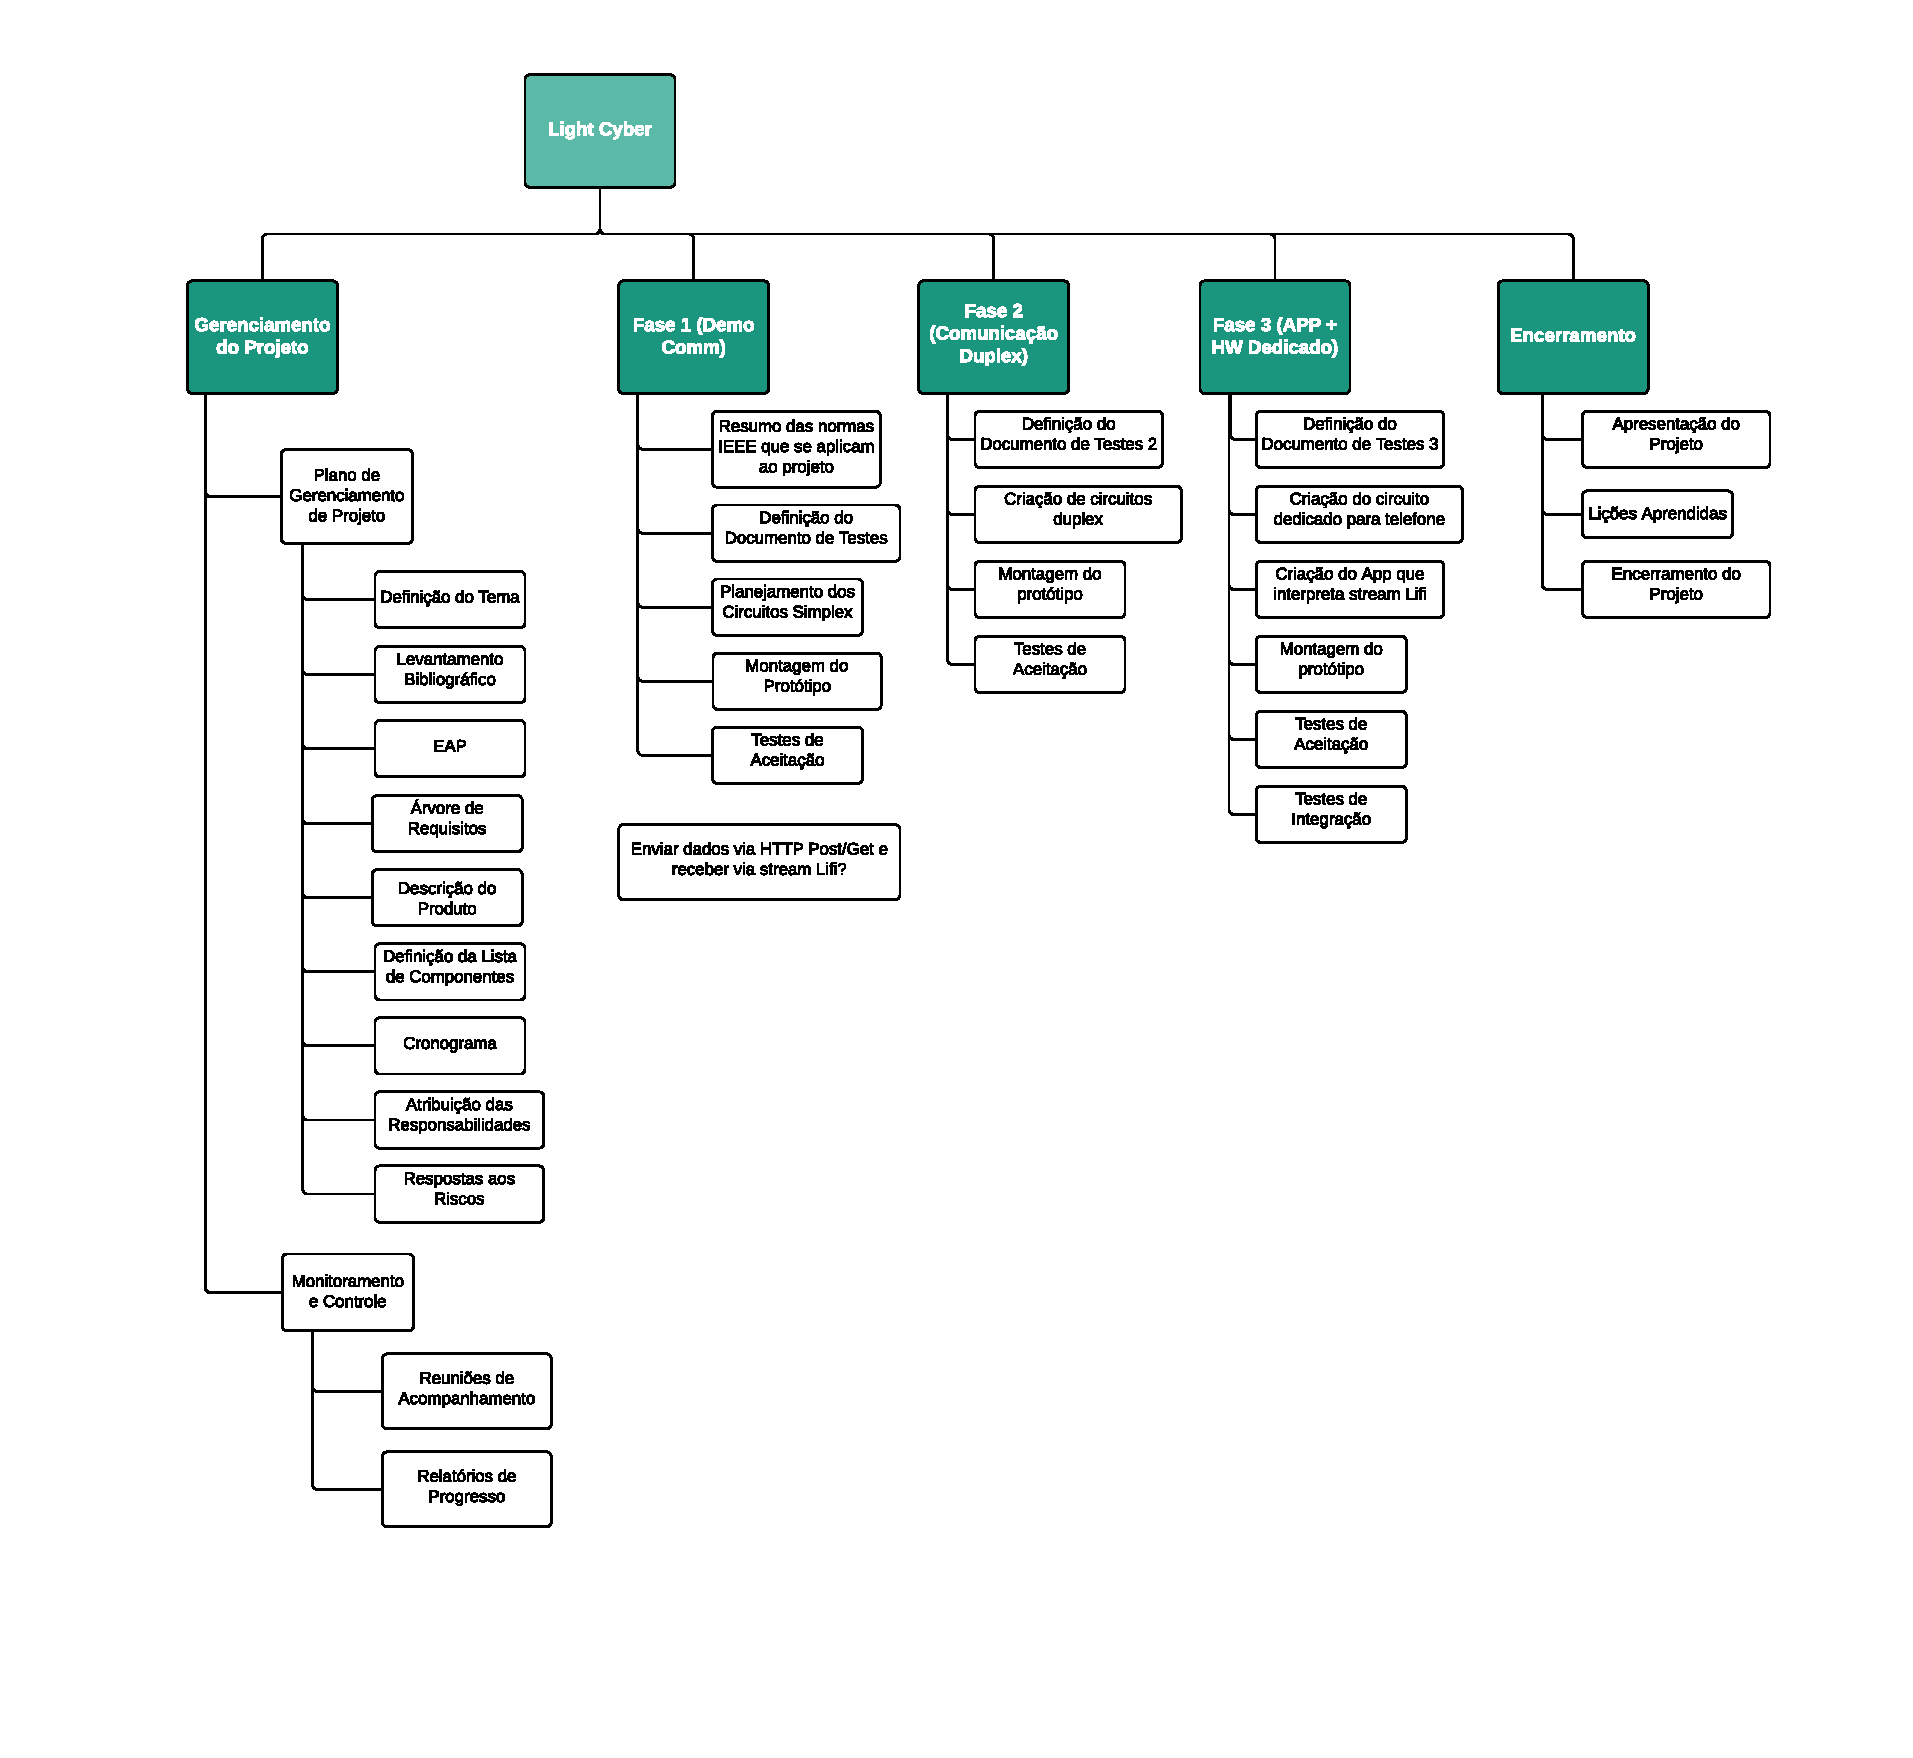
\includegraphics[width=1.0\textwidth, trim={1cm 1cm 1cm 1cm}, clip]{EAP.pdf}}
	\end{figure}
	
	% ---
	\subsection{Cronograma}\label{subsec-cronograma}
	% ---
	
	O cronograma do projeto foi planejado a partir dos pacotes de trabalho definidos na Estrutura Analítica de Projeto. Os participantes então fizeram reuniões para estimar o tempo, com a aplicação dessas estimativas a um calendário, considerando ainda as datas de entrega oficiais da disciplina. Com todas as estimativas feitas, o projeto tem a primeira e segunda fase com duração até o fim de Julho, com intuito de adiantar tanto a documentação quanto a implementação, como pode-se observar no diagrama de Gantt  \autoref{fig_gantt} abaixo.
	
	\begin{figure}[h!]
		\caption{\label{fig_gantt} Diagrama de Gantt do projeto LiCy}
		\centering
		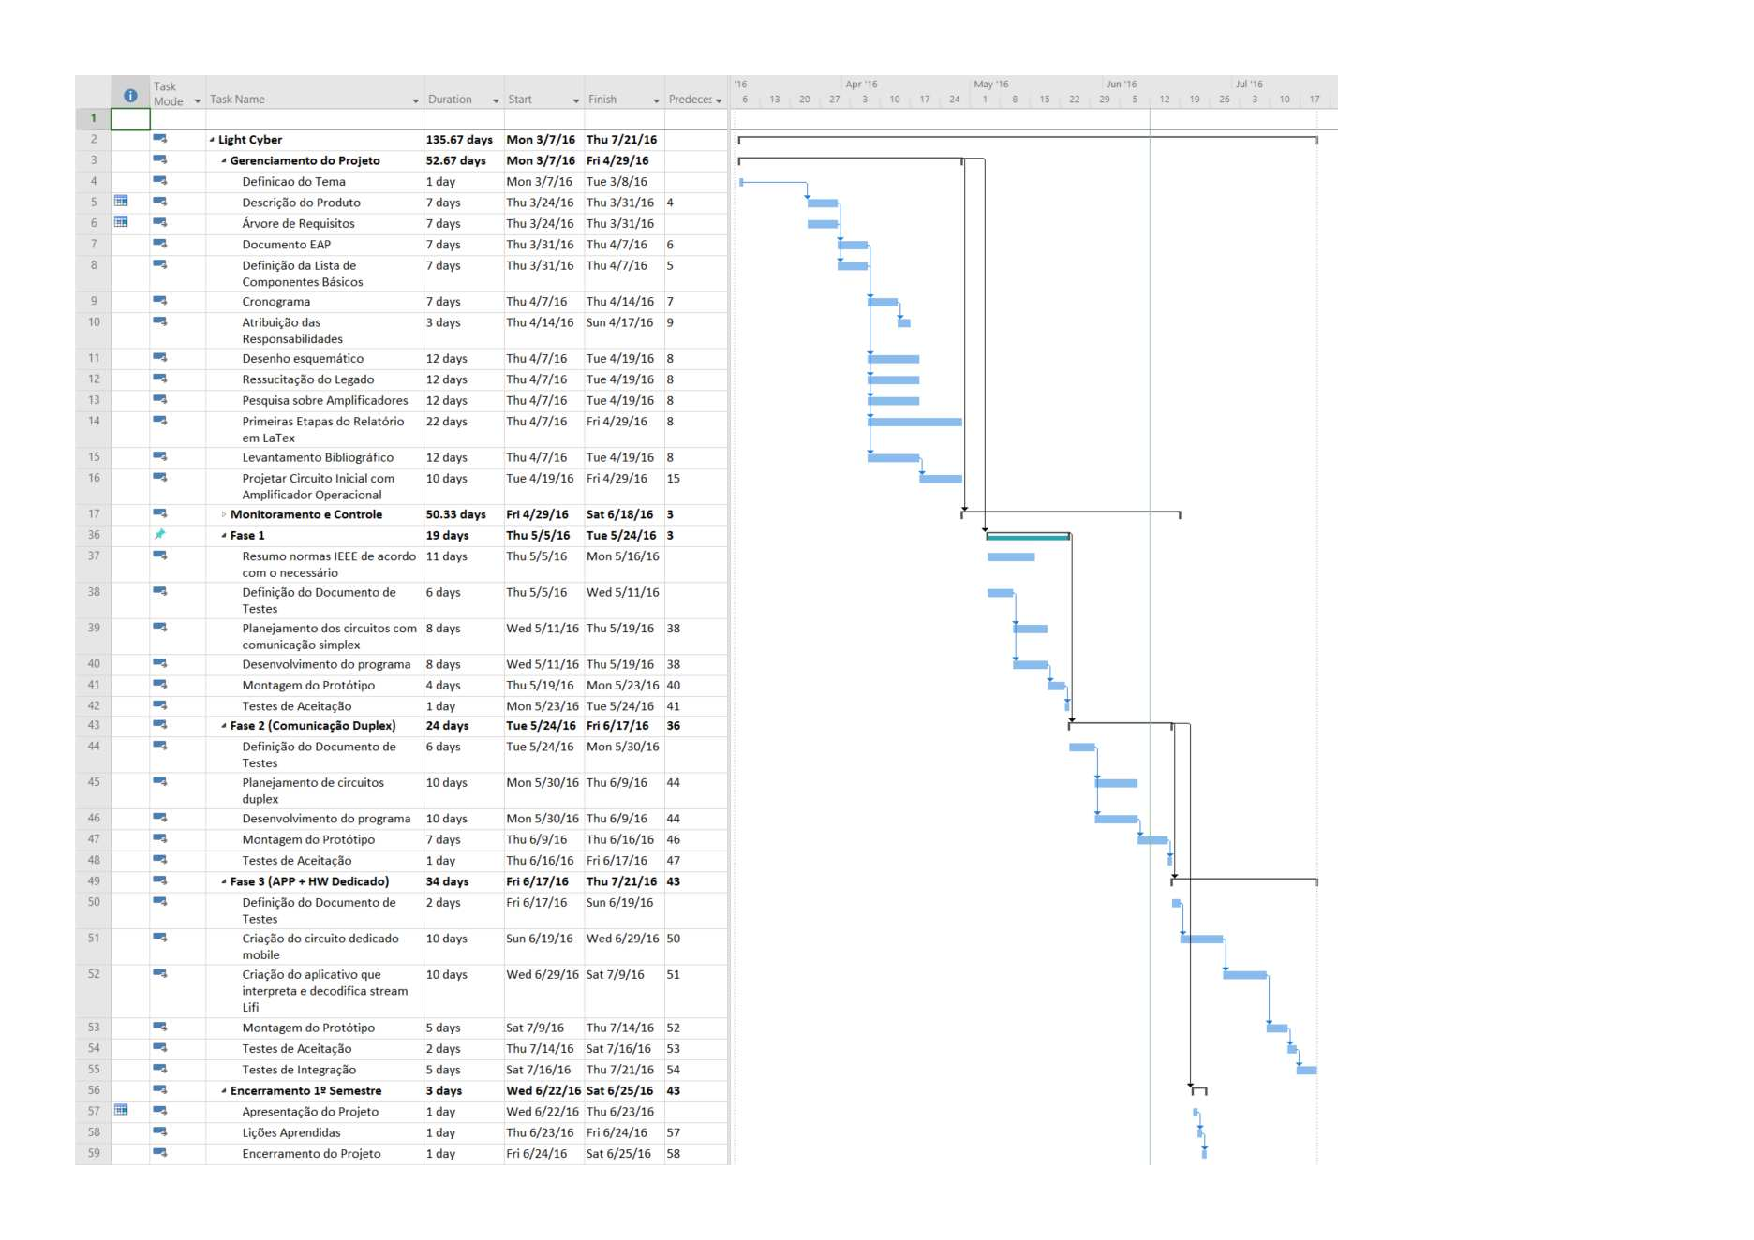
\includegraphics[width=1.0\textwidth, trim={1cm 1cm 7cm 1cm}, clip]{gantt.pdf}
	\end{figure}
	
	% ---
	\subsection{Requisitos}\label{subsec-requisitos}
	% ---
	
	Os requisitos foram divididos primeiramente em funcionais e não-funcionais. Além disso, existem outras divisões relacionadas a hardware, software, estética e módulos do sistema. Para cada requisito foi dado um peso, conforme avaliação da relevância deste requisito para este projeto, de modo que no topo da árvore haja uma soma equivalente a 1.
	
	% ---
	\subsubsection{Requisitos Funcionais}\label{subsubsec-requisitos-func}
	% ---
	\textbf{Requisitos de hardware:} é importante observar que estes dividem-se entre a lamparina, que serve de ponto de acesso, e o módulo de celular, com pesos iguais entre os dois, já que a comunicação é bilateral e ambos têm importância equivalente. Há requisitos em comum entre esses subsistemas:
	\begin{itemize}  
		\item Estar de acordo com a norma IEEE 802.15.7, que tem o peso mais alto, já que compreende o escopo principal deste trabalho, que é implementá-la;
		\item Utilização da FPGA e de um microcontrolador, para implementar as camadas física, MAC\footnote{ Media Access Control, ou camada de enlace.},  TCP, IP e de aplicação. As justificativas para o uso desses dois componentes segue nos próximos itens;
		\item Comunicação full-duplex um a um, diz respeito a garantir a bilateralidade da comunicação entre dois nós, com recepção e transmissão independentes nas duas partes;
		\item Utilizar LED e fotodiodo, para transmitir e receber, respectivamente, os dados modulados através da luz;
		\item Filtrar a luz ambiente, que é primordial para que a recepção seja bem sucedida, do contrário pode haver muita interferência da luz que não tenha o LED como fonte. Deve fazer com que o sistema se aproxime ao máximo de um cenário ideal, onde há apenas um LED e um fotodiodo num ambiente escuro.
	\end{itemize}
	
	A lamparina possui requisitos de hardware próprios, incluindo funcionar como Access Point, ou seja, fornecer acesso a uma fonte de dados, que pode ser uma rede local, um computador, a internet, entre outros. Outro requisito importante e complementar a este, é a conexão desse módulo a alguma dessas fontes através de uma interface Ethernet.
	
	Já o módulo de celular tem como requisitos de hardware exclusivos o consumo de energia através de uma bateria e a conexão ao celular através da interface USB.	
	
	\textbf{Requisitos de software:} dividem-se entre a lamparina, o módulo de celular e o aplicativo, utilizado para receber e enviar dados para este módulo. Existem requisitos que são complementares às funções de hardware, porém correspondentes às soluções de software adotadas, como a implementação da norma IEEE 802.15.7 e a comunicação full-duplex um a um. Além destes, existem os requisitos de software comuns tanto à lamparina, ou Access Point Li-Fi, como ao módulo de telefone:
	
	\begin{itemize}  
		\item Lidar com luz ambiente, ou seja, minimizar a interferência causada por ela, e mitigar o efeito de erros, corrigindo ou descartando pacotes que os contenham;
		\item Transmissão de dados pelo módulo de celular e recepção pela lamparina, representam o mesmo fluxo de dados mas de dois lados da comunicação;
		\item Transmissão de dados e multimídia pela lamparina e recepção destes pelo módulo de celular;
	\end{itemize}
	
	O módulo de celular possui um requisito de software exclusivo, que é a utilização de um protocolo conhecido para se comunicar com o celular via USB. Do outro lado, o lamparina deve se conectar à internet e lidar com os pacotes que chegarem desta rede. 
	
	Além desses requisitos, existem também aqueles referentes ao aplicativo de celular, que deve decodificar os dados recebidos via USB, deve ser desenvolvido a fim de funcionar no sistema operacional Android e deve exibir vídeos, imagens ou websites.

	\begin{figure}[h!]
		\caption{\label{fig_req1} Requisitos Funcionais }
		\centering
		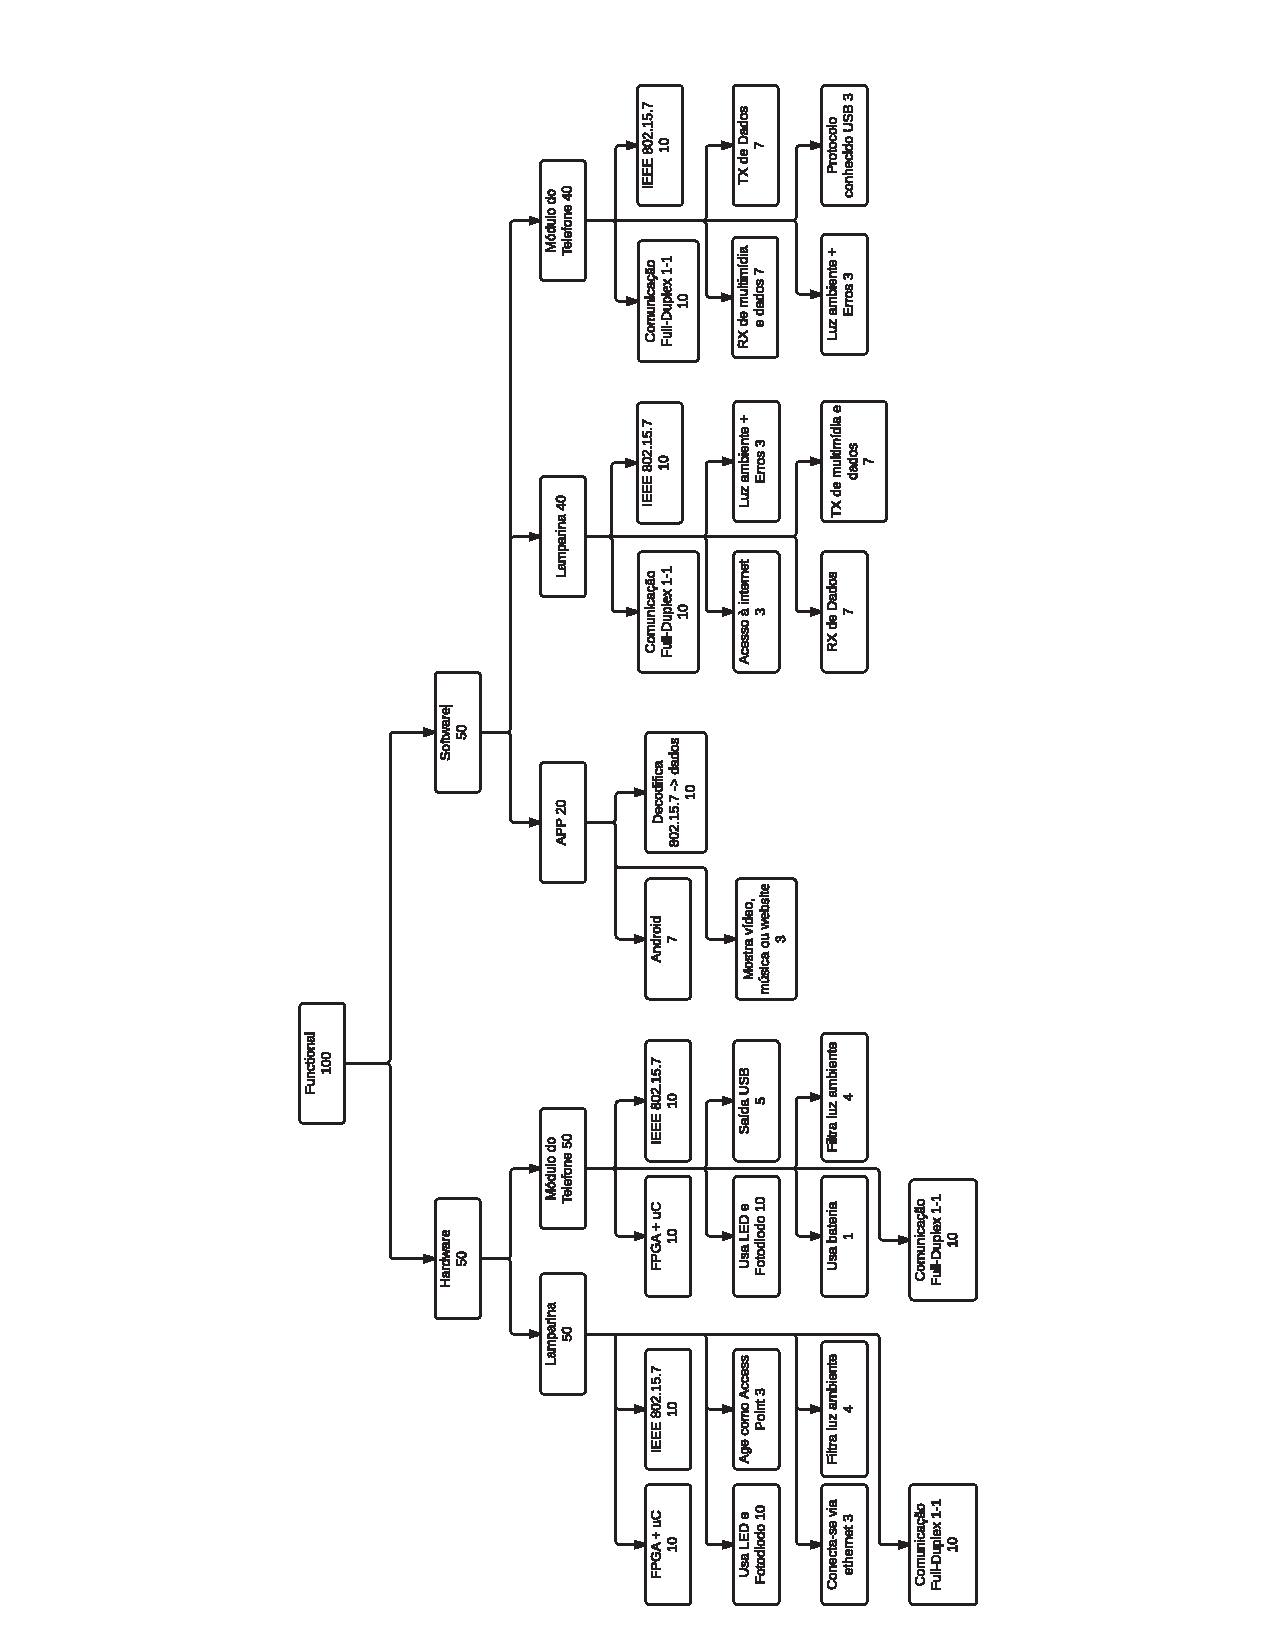
\includegraphics[width=0.5\textwidth, trim={5cm 0.5cm 3cm 1.3cm}, clip]{ReqTree1.pdf}
	\end{figure}
	
	\subsubsection{Requisitos Não-Funcionais}\label{subsubsec-requisitos-nfunc}
	\textbf{Transmissão de dados:} Deve-se principalmente manter a velocidade da banda conforme a especificação da norma IEEE 802.15.7 para cada camada PHY correspondente. É também primordial garantir a confiabilidade na comunicação, ou seja, garantir que os bits recebidos estão corretos e quando possível e necessário, corrigi-los, com as limitações que serão discutidas posteriormente no que diz respeito à norma (ver módulos de codificação e decodificação). Além disso, há um requisito de segurança, que equivale a evitar a possibilidade de vazamento de dados para terceiros, ou até a intromissão de mensagens indesejadas na comunicação.
	\textbf{Modulação de luz:} O requisito mais importante é garantir o funcionamento do sistema a uma distância de até 1 metro, considerando uma aplicação residencial do produto. Secundariamente, há o requisito de manter um baixo consumo de energia, que apesar de fundamental em produtos de tecnologia da informação, foge do escopo deste estudo.
	
	\begin{figure}[h!]
		\caption{\label{fig_req2} Requisitos Não Funcionais}
		\centering		%  trim={<left> <lower> <right> <upper>} 
		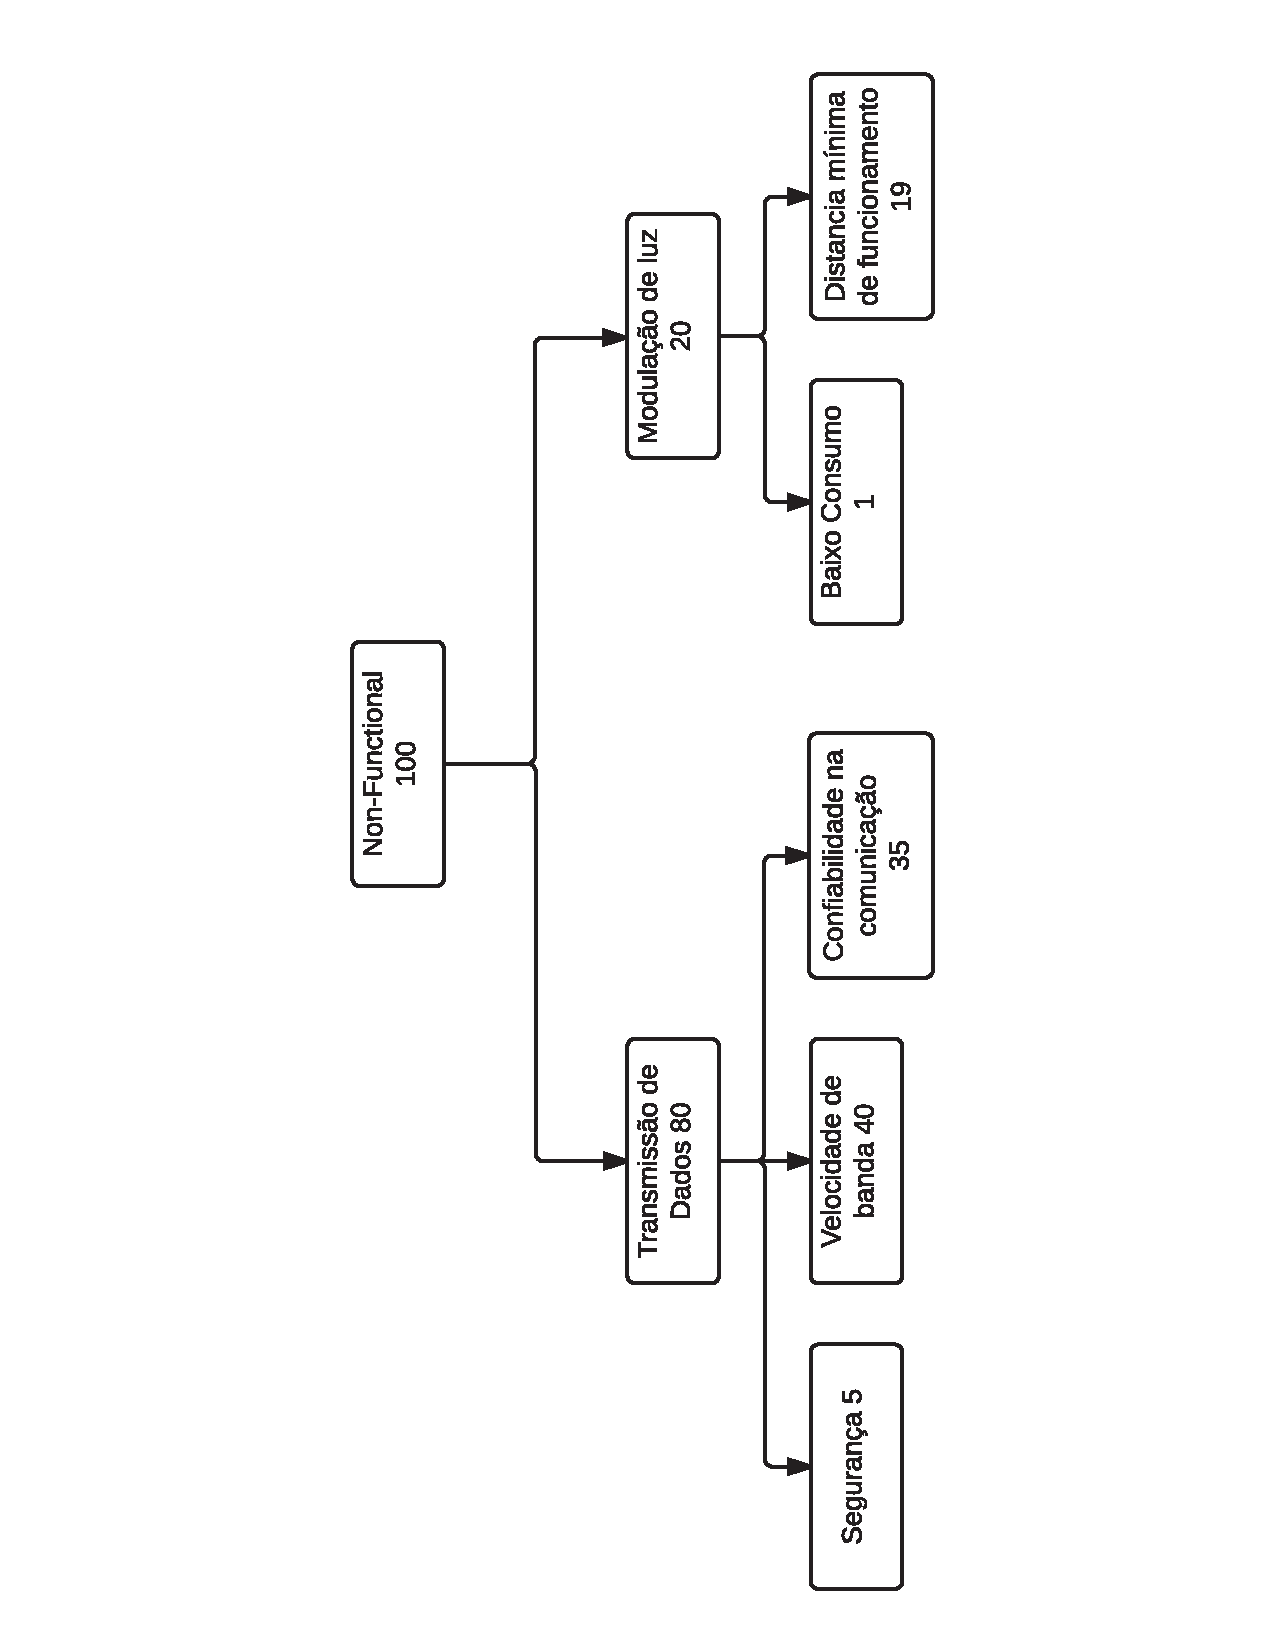
\includegraphics[width=0.9\textwidth, trim={1cm 5.5cm 1cm 6cm}, clip]{ReqTree2.pdf}
	\end{figure}
	
	\begin{figure}[h!]
		\caption{\label{fig_req3} Outros Requisitos}
		\centering
		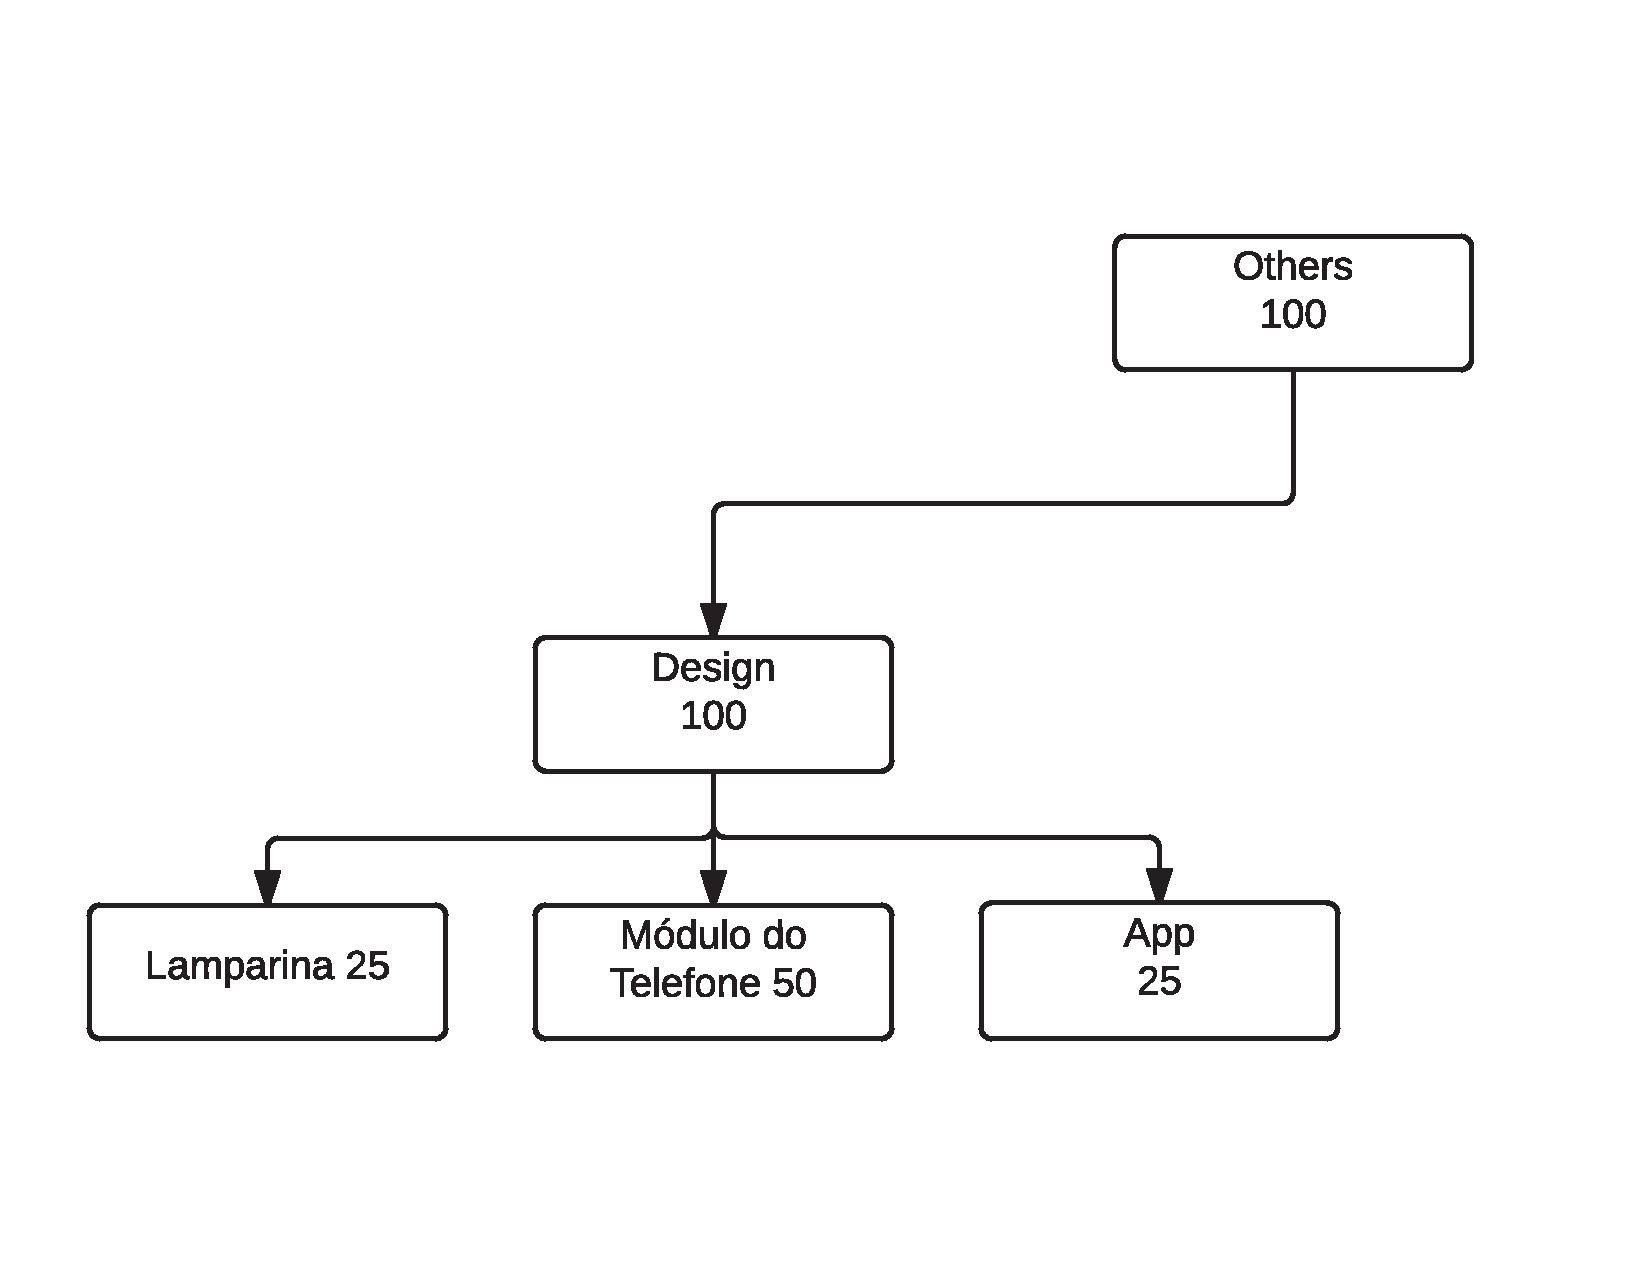
\includegraphics[width=0.7\textwidth, trim={1cm 4cm 3cm 4cm}, clip]{ReqTree3.pdf}
	\end{figure}
	
	% ---
	\section{Norma IEEE 802.15.7}\label{sec-norma}
	% ---
	
	A norma 802.15.7 estabelece um padrão para comunicação via luz, no que se diz respeito à definição de topologias de rede, codificação da informação, divisão das camadas da arquitetura do sistema de comunicação, ordem e conteúdo de cabeçalhos para cada camada e definições sobre a segurança do \textit{link}. A arquitetura de um sistema LiFi completo está definida na \autoref{fig_architecture}.
	
	\begin{figure}[htb]
		\caption{\label{fig_architecture} Arquitetura de dispositivos VPAN}
		\centering
		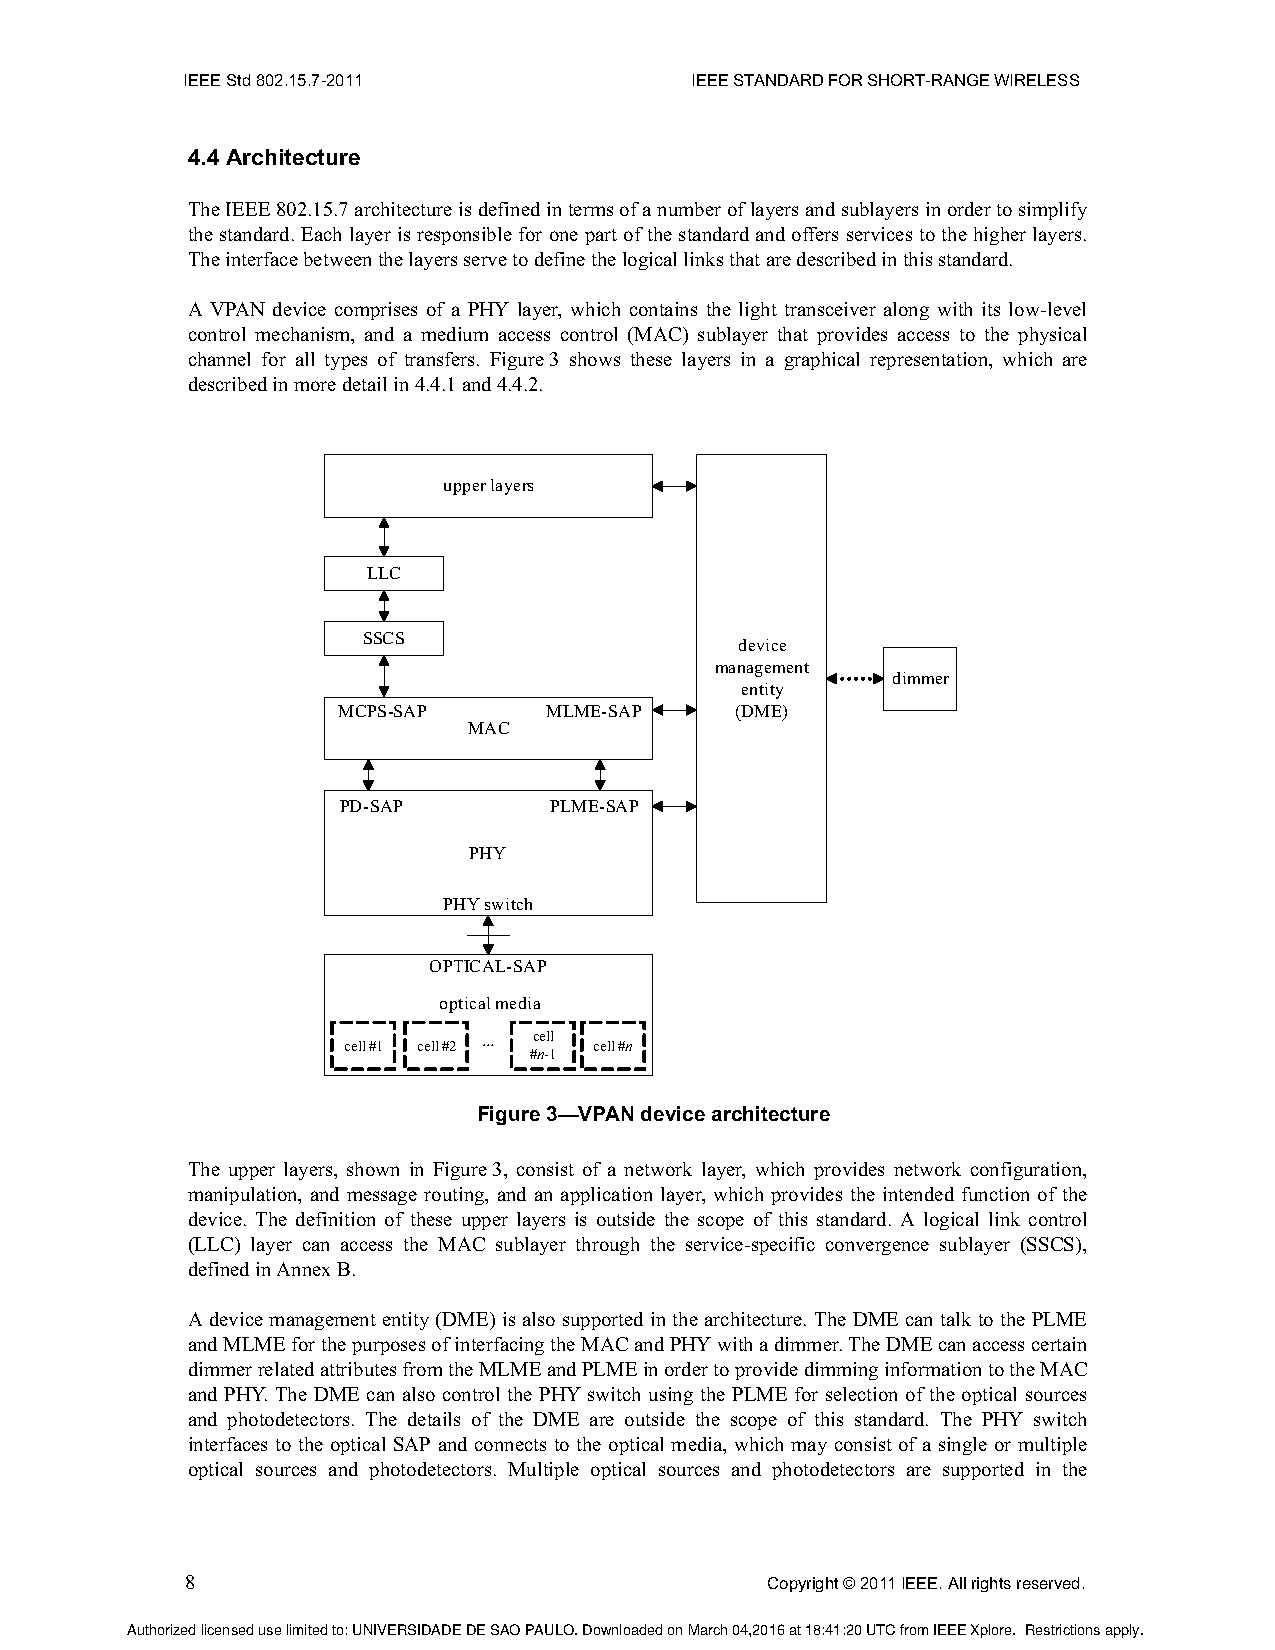
\includegraphics[width=0.5\textheight,trim={5.5cm 9.6cm 5.3cm 7cm}, clip]{pag31.pdf}
		\legend{Fonte: IEEE 802.15.7}
	\end{figure}

%	\begin{figure}[htb]
%		\caption{\label{fig_transmission_simple_blocs} Diagrama de blocos simplificado da transmissão da camada PHY I}
%		\centering
%		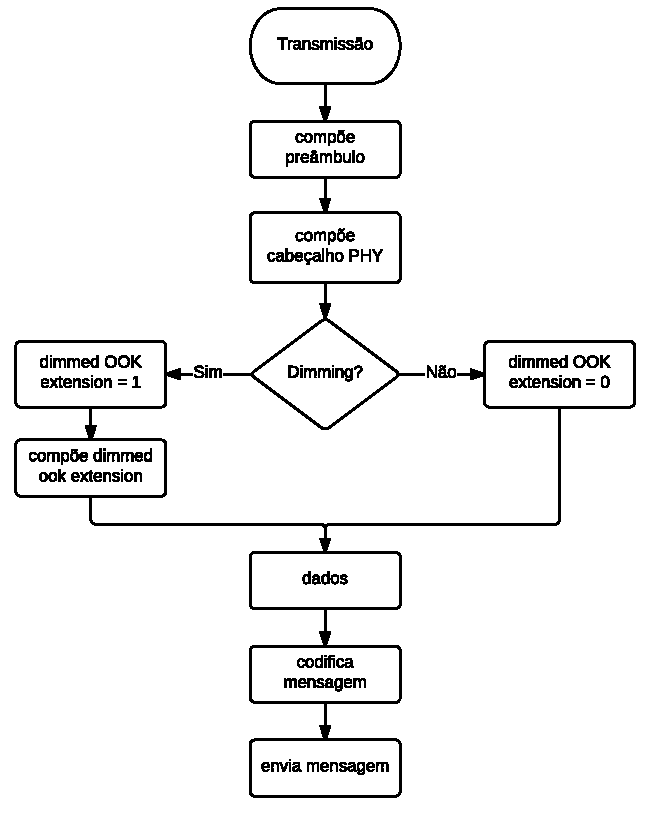
\includegraphics[width=0.4\textheight]{transmissao-blocos-simplificado.pdf}
%	\end{figure}

	\subsection{Transmissão}
	
	Nessa seção será discorrido o processo de transmissão de dados via luz, levando em conta códigos cíclicos de correção de erro, redução de erros em burst e protocolos RLL, especificados pela norma IEEE. Para realizar a transmissão, é necessário passar pelas etapas do diagrama abaixo:
		
		\begin{figure}[htb]
			\caption{\label{fig_transmission_phy1} Diagrama de blocos da codificação da mensagem}
			\centering
			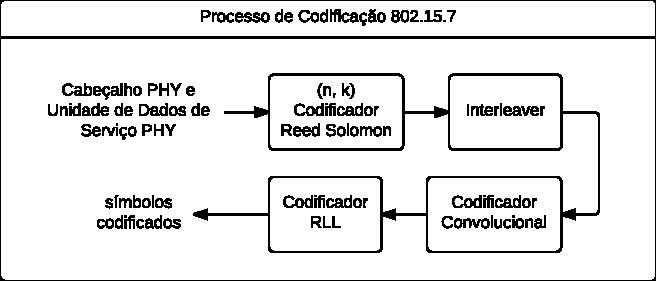
\includegraphics[width=0.6\textheight]{PHY1-transmission.pdf}
			\legend{Fonte: @todo figura 126}
		\end{figure}
		
	Para que os dados transmitidos sejam corretamente recebidos, a norma estabelece algumas regras para codificação da mensagem, a fim de garantir recuperação de erros, redução de erros em burst, maior facilidade na sincronia do clock, entre outros detalhes. A \autoref{fig_transmission_phy1} ilustra os passos necessários para compor a mensagem antes de sua transmissão. Os passos estarão detalhados nas seções a seguir.
	
	\subsubsection{Codificação Reed Solomon}
	
	Com intuito de adicionar redundância de informação na mensagem, a norma estabelece um mecanismo de correção de erros antecipada (FEC). Mais especificamente, o código de Reed Solomon. 
	
	\paragraph{Campos de Galois}

		\cite{nasa-rs1}
		
	\paragraph{Operações}
	
	
	\subsubsection{Codificação RLL}
	
	Para a primeira camada de implementação PHY I, será escolhida codificação RLL Manchester, que é codifica os bits 0 e 1 de acordo com a \autoref{tabela_cod_manchester}. Após 
	
	\begin{table}[ht]
		\caption{Codificação Manchester}
		\centering
		\begin{tabular}{c c}
			\hline
			bit & manchester symbol \\ \hline
			0 & 01 \\
			1 & 10 \\ \hline
		\end{tabular}
		\label{tabela_cod_manchester}
		\legend{Fonte: Tabela XYZ da norma 802.15.7}
	\end{table}
	
	\subsubsection{Interleaver}
	
	\subsubsection{Puncture}
	
	\subsubsection{Padding}
		
	\subsection{Recepção}
	
	% ---
	\section{Hardware}\label{sec-hardware}
	% ---
	
	Explica as escolhas feitas de hardware.
	
	% ---
	\subsection{FPGA}\label{hard-fpga}
	% ---
	
	FPGA (Field-Programmable Gate Array) é uma tecnologia que utiliza chips de silício reprogramáveis para obter circuitos customizáveis, latência a nível de hardware\footnote{muito muito rápido} e vazão muito alta\footnote{devido ao alto grau de paralelismo}. No projeto LiCy, como o fluxo de informações é muito alto (requisito de projeto de 1Gbps), é necessário realizar múltiplos processos ao mesmo tempo para lidar com os dados:
	
	\begin{itemize}  
		\item Recebimento/Transmissão de dados
		\item Cálculo de paridade
		\item Correção de erros\footnote{apenas para recebimento}
		\item (De)codificação de dados
	\end{itemize}
	
	\begin{table}[htbp]
		\caption{\label{tab_phy1} Modos de operação da camada PHY I de Li-Fi}

		\centering
		%  trim={<left> <lower> <right> <upper>} 
		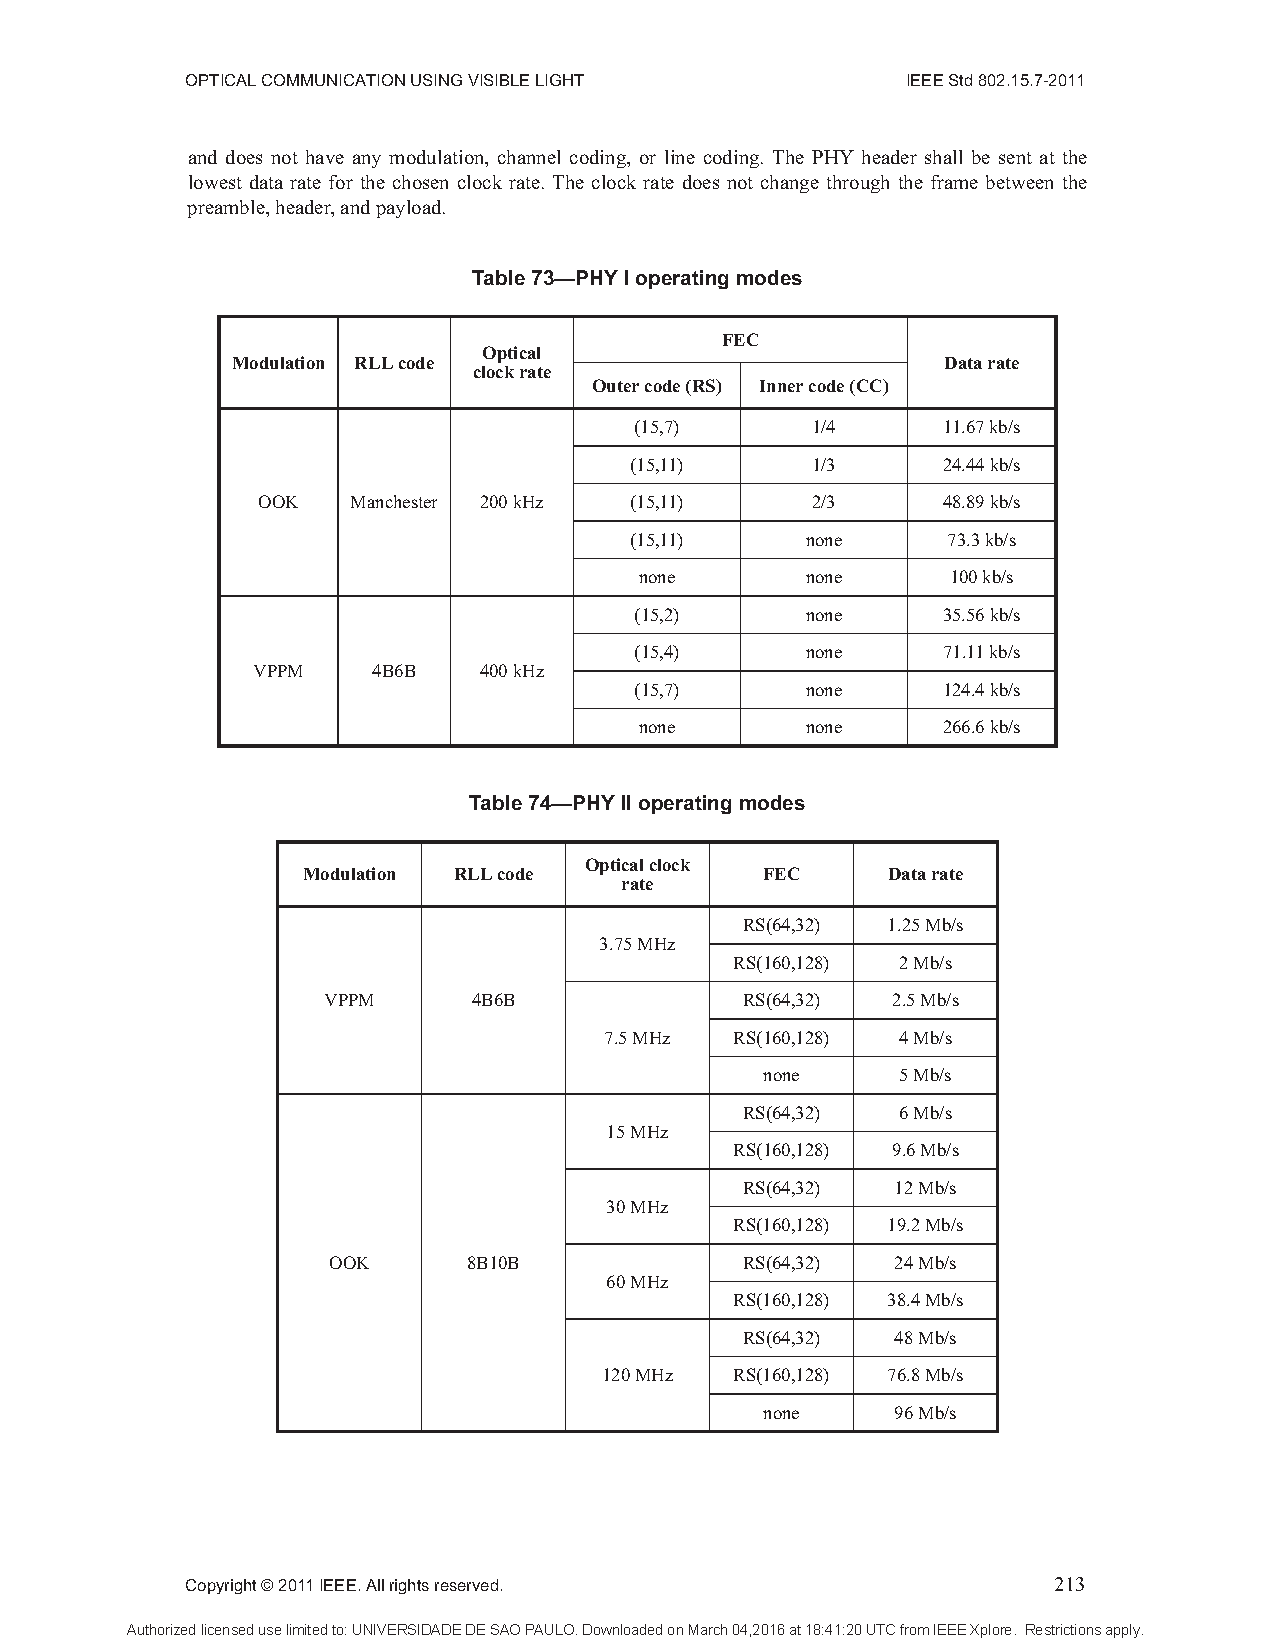
\includegraphics[clip, trim=37mm 151mm 36mm 51mm,  width=0.7\textwidth]{pag213.pdf}
		\legend{Fonte: IEEE 802.15.7}
	\end{table}
	
	\begin{table}[htbp]
		\caption{\label{tab_phy2} Modos de operação da camada PHY II de Li-Fi}
		\centering
			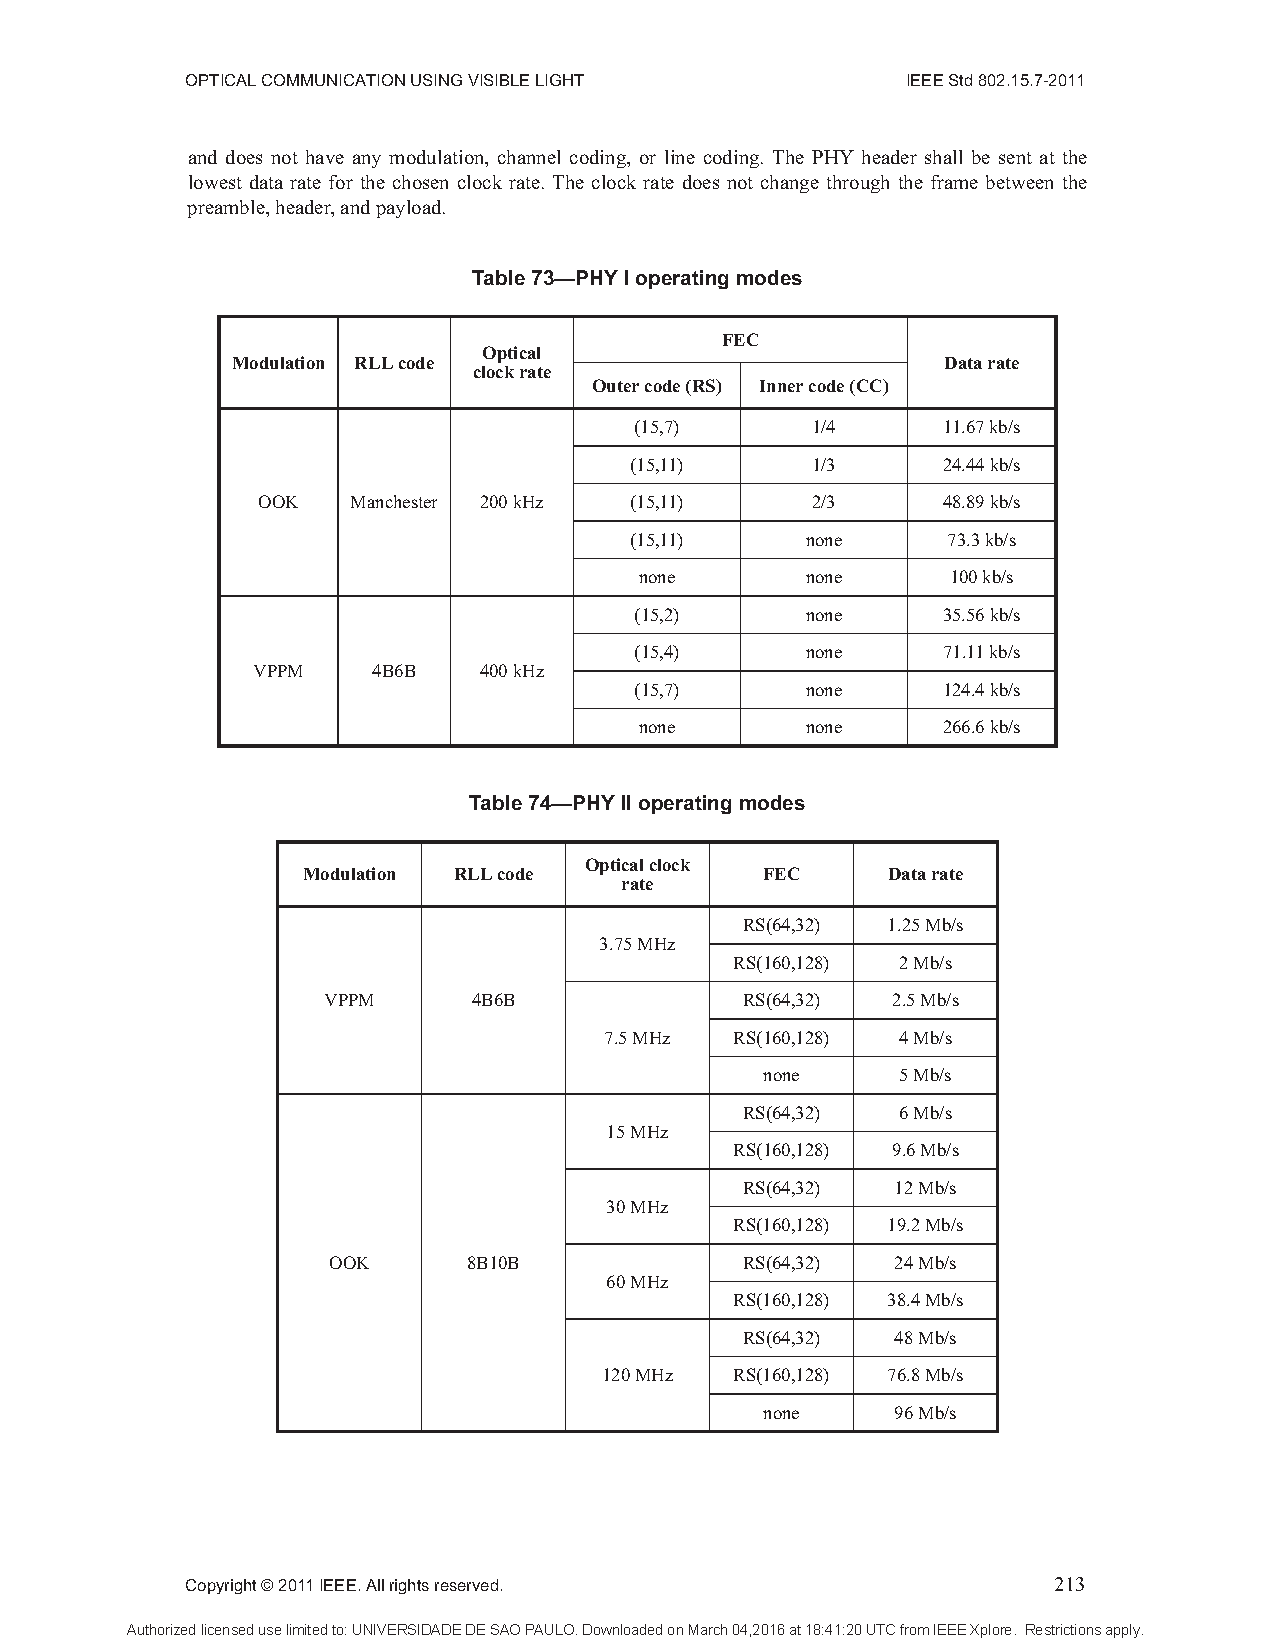
\includegraphics[clip, trim=46.55mm 36.79mm 46.74mm 142.30mm,  width=0.7\textwidth]{pag213.pdf}
		\legend{Fonte: IEEE 802.15.7}
	\end{table}

	Essa tecnologia é ideal para criar protótipos de circuitos digitais. Existe neste caso a facilidade de mudar o arranjo de componentes e vias de dados, bem como a possibilidade de simulá-los e depurá-los antes mesmo de gravar as configurações no hardware. Estes são elementos chave para a criação de um ambiente controlado, para testar as funcionalidades do produto desenvolvido. Sendo assim, um dos fatores que mais motivou a escolha dessa tecnologia neste projeto.
	
	O projeto de uma FPGA possui características que anteriormente estavam associadas a sistemas baseados em processadores. Uma delas é o uso de ferramentas e interfaces de alto nível, usando diagramas de bloco representando comportamentos e linguagens de descrição de hardware (na sigla em inglês, HDL), que no entanto diferem em muito de linguagens de programação como C. 
	
	A principal vantagem do uso de uma FPGA em relação a microcontroladores está na independência das operações de processamento, que por estarem em circuitos paralelos não precisam dividir recursos, como um mesmo núcleo por exemplo. Entretanto, o alto grau de paralelismo pode resultar em maiores desafios como garantir o sincronismo e lidar com inconsistência de dados no nível de circuito. Ainda assim, é preferível neste projeto lidar com esses desafios para se beneficiar do ganho em latência e vazão de dados.
	
	
	\begin{comment}
	--
	 O que é um FPGA?  http://www.ni.com/white-paper/6984/pt/ Publicação: Dez 21, 2011 | 1 Avaliação | 4,00 de 5 | Read in English  | Imprimir
	 
	 FPGAs são chips de silício reprogramáveis que usa blocos lógicos programáveis pré-construídos que tem recursos de roteamento, você pode configurar esses chips para implementar funcionalidades personalizadas de hardware, sem nunca ter que pegar em uma placa de montagem ou ferro de solda. Você desenvolve tarefas de computação digital em software e as compila em um arquivo de configuração ou bitstream que contém informações sobre como os componentes devem ser ligados entre si. Além disso, os FPGAs são totalmente reconfiguráveis e imediatamente assumem uma nova "personalidade" quando você recompila uma nova configuração de circuito. No passado, a tecnologia FPGA só estava disponível para engenheiros com uma profunda compreensão do projeto de hardware digital. O surgimento de ferramentas de projeto de alto nível, no entanto, está mudando as regras da programação FPGA, com as novas tecnologias que convertem diagramas de blocos gráficos ou mesmo código em C em circuitos de hardware digital.
	 
	 A adoção de chips FPGA em todos os setores é dirigida pelo fato dos FPGAs combinarem as melhores partes do ASIC a sistemas baseados em processador. Os FPGAs oferecem confiabilidade  e velocidade na temporização por hardware, mas não exigem grandes volumes para justificar o grande gasto inicial de um projeto ASIC personalizado. O silício reprogramável também tem a mesma flexibilidade de um software rodando em um sistema baseado em processador, mas não é limitado pelo número de núcleos de processamento disponível. Ao contrário de processadores, os FPGAs são verdadeiramente paralelos por natureza, de modo que diferentes operações de processamento não têm que consumir os mesmos recursos. Cada tarefa independente de processamento é atribuído a uma seção dedicada do chip, e pode funcionar de forma autônoma, sem qualquer influência de outros blocos lógicos. Como resultado, o desempenho de uma parte da aplicação não é afetada quando um processamento adicional é inserido.
	 --
	
		
	Explicação do porquê foi escolhido FPGA
	http://electronics.stackexchange.com/questions/4382/fpgas-vs-microcontrollers
	
	Designing for an FPGA requires a Hardware Description Language (HDL). HDLs are absolutely nothing at all like C. Whereas a C program is a sequential series of instructions and must contort itself to achieve parallel execution, an HDL describes a concurrent circuit and must contort itself to achieve sequential execution. It is a very different world and if you try to build a circuit in an FPGA while thinking like a software developer it will hurt.
	
	An MCU is time-limited. In order to accomplish more work, you need more processor cycles. Clocks have very real limits to their frequencies, so it's easy to hit a computational wall. However, an FPGA is space-limited. In order to accomplish more work, you merely add more circuits. If your FPGA isn't big enough, you can buy a bigger one. It's very hard to build a circuit that can't fit in the largest FPGA, and even if you do there are app notes describing how to daisy chain FPGAs together.
	
	FPGAs focus way more on parallel execution. Sometimes you have to worry about how long your MCU's ISR takes to service the interrupt, and whether you'll be able to achieve your hard-real-time limits. However, an in FPGA there are lots of Finite State Machines (FSM) running all the time. They are like "femto-controllers", like little clouds of control logic. They are all running simultaneously, so there's no worrying about missing an interrupt. You might have an FSM to interface to an ADC, another FSM to interface to a microcontroller's address/data bus, another FSM to stream data to a stereo codec, yet another FSM to buffer the dataflow from the ADC to the codec...You need to use a simulator to make sure that all the FSMs sing in harmony. If any control logic is off by even a single clock cycle (and such mistakes are easy to make) then you will get a cacophony of failure.
	
	FPGAs are a PCB layout designer's wet dream. They are extremely configurable. You can have many different logic interfaces (LVTTL, LVCMOS, LVDS, etc), of varying voltages and even drive strengths (so you don't need series-termination resistors). The pins are swappable; have you ever seen an MCU address bus where the pins were scattered around the chip? Your PCB designer probably has to drop a bunch of vias just to tie all the signals together correctly. With an FPGA, the PCB designer can then run the signals into the chip in pretty much any order that is convenient, and then the design can be back-annotated to the FPGA toolchain.
	
	--
	Often FPGAs get used specifically to do tasks a microcontroller cannot do efficiently, such as highly parallel or low latency operations, operating in multiple clock domains, or doing custom logic at hardware speeds. As such, they'll do the heavy lifting, and you rarely need an MCU to be central to the design - they may be moved to management positions, such as loading the configuration bitstream. An example of this is the PIC or ARM in the Minimig, which implements the storage interface.
	
	--
	http://electronics.stackexchange.com/questions/97277/when-can-fpgas-be-used-and-microcontrollers-dsps-not
	
	The key thing to consider is throughput and latency requirements. A microcontroller can service an interrupt (very roughly) once per microsecond. It can only service one interrupt at once. If you need to process it in an elaborate way, that limits how many you can service in a particular time.
	
	With an FPGA, you can generally respond to an input event immediately (well, on the next clock cycle). You can have lots of processing units in parallel. If you know that your filter takes 20 cycles, that's entirely independant of anything else going on.
	
	Highly-parallel integer intensive computation works best on FPGAs, especially if there's complex data dependencies. However, they don't have a lot of onboard memory; you can add some DRAM to the side but at the cost of latency.
	\end{comment}
	
	% ---
	\subsubsection{Opções Consideradas}\label{fpga-options}
	% ---
	
	Explicação de quais foram as opções consideradas.
	
	% ---
	\subsubsection{Tabela Comparativa}\label{fpga-table}
	% ---
	
	Tabela de opções consideradas.
	
	% ---
	\subsection{Microcontrolador}\label{hard-uc}
	% ---
	
	O microcontrolador escolhido foi o Photon.
	
	\begin{figure}[htb]
		\caption{\label{fig_photon} Desenho esquemático do microcontrolador Photon}
		\begin{center}
			%  trim={<left> <lower> <right> <upper>} 
			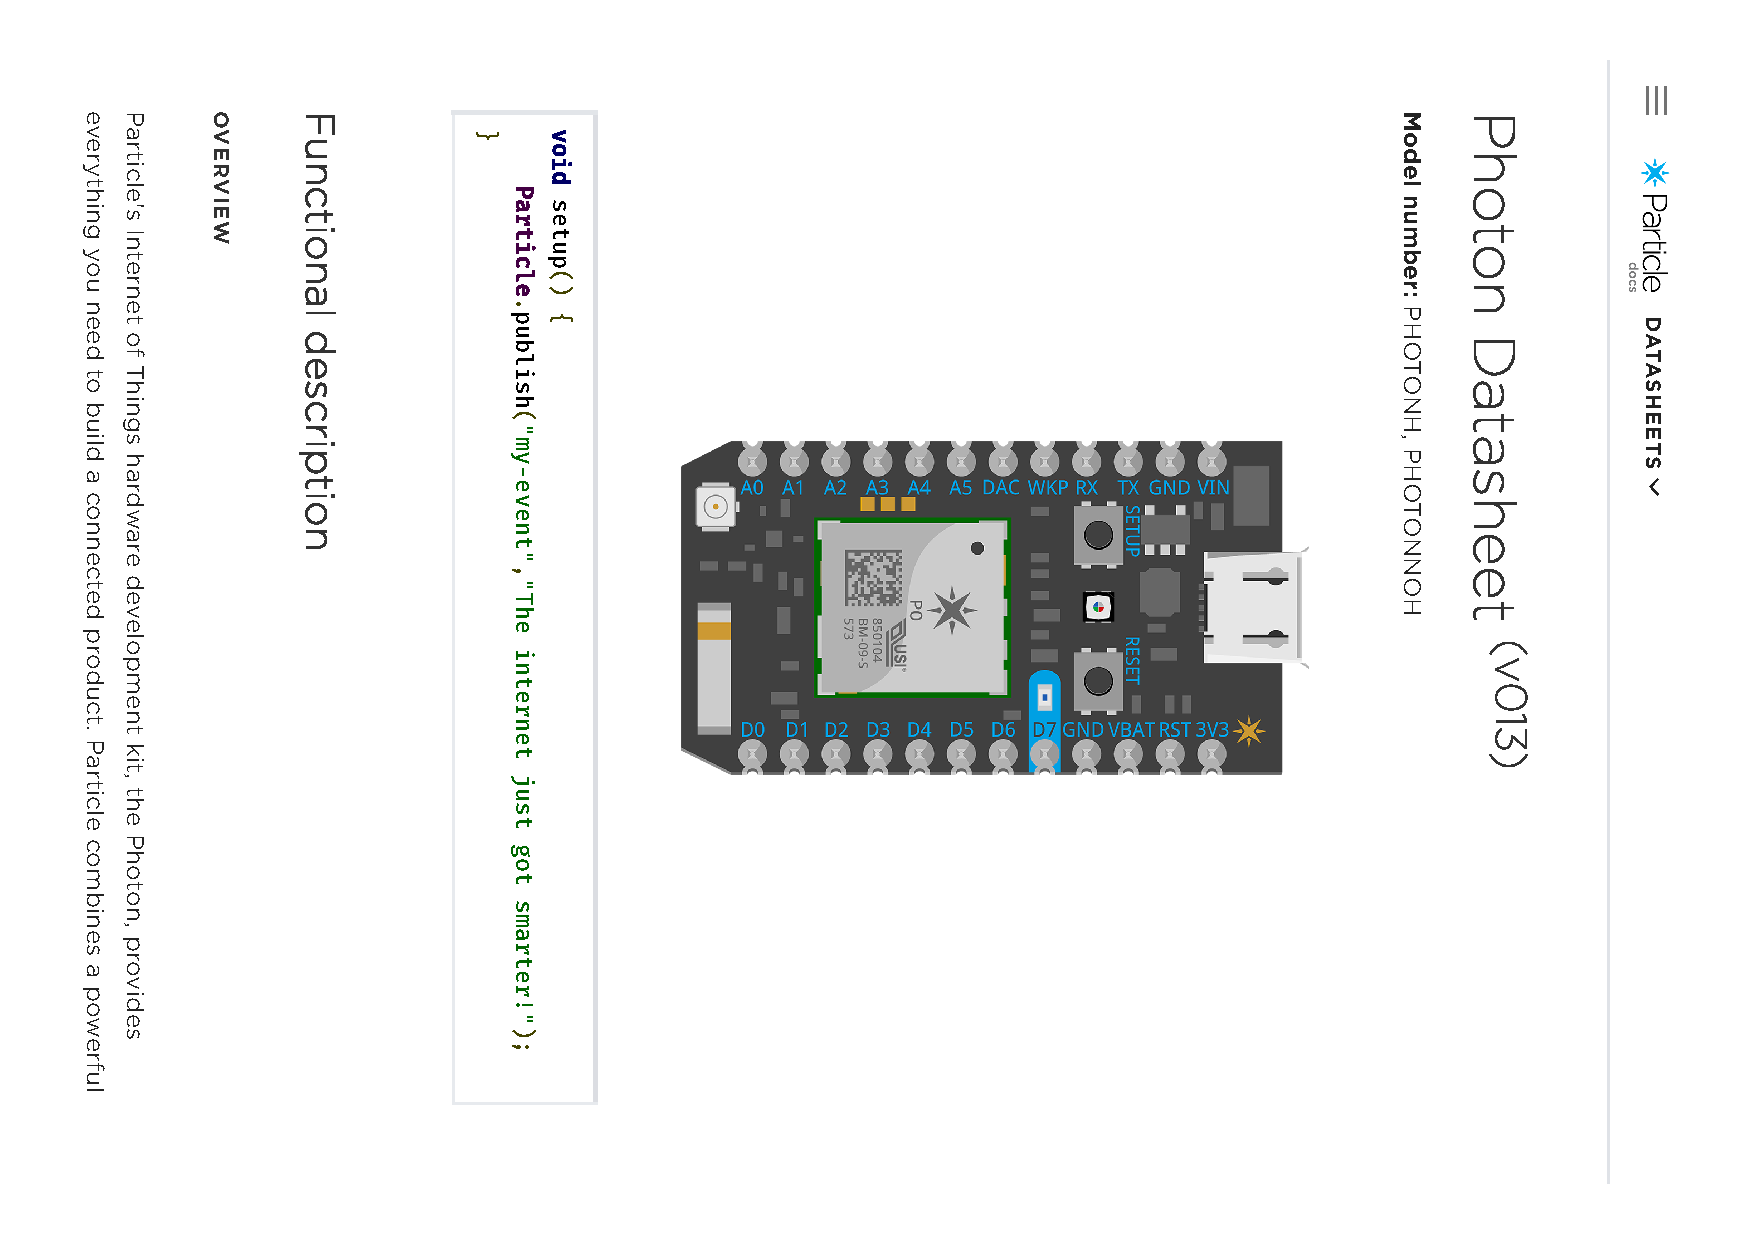
\includegraphics[width=0.5\textheight, trim={11.7cm 7.9cm 7.8cm 7.4cm}, clip]{photon.pdf}
		\end{center}
		\legend{Fonte: Particle Docs}
	\end{figure}

	
	Explicação do porquê foi escolhido microcontrolador
	
	Conexão com fgpa e microcontrolador
	The best way to connect them is to use an MCU with an external address and data bus. Then you can simply memory map the FPGA circuits into the MCU, and add your own "registers" that each have their own address. Now the FPGA can add custom peripherals, like a 32-bit timer that can latch all 4 bytes at once when the first byte is read to prevent overflows between 8-bit reads. You can also use it as glue logic to memory map more peripherals from other chips, like a separate ADC.
	
	
	% ---
	\subsubsection{Opções Consideradas}\label{uc-options}
	% ---
	
	% ---
	\subsubsection{Tabela Comparativa}\label{uc-table}
	% ---
	
	% ---
	\subsection{LED}\label{hard-led}
	% ---
	
	De acordo com a \autoref{tab_phy1} e \autoref{tab_phy2}, para cada camada física implementada é necessário suportar uma frequência de oscilação luminosa mínima:
	
	\begin{itemize}
		\item PHY I: 400kHz
		\item PHY II: 120MHz
	\end{itemize} 
	
	O LED escolhido para a transmissão deverá então suportar essas frequências de acordo com a implementação de cada camada. 
	
	O componente \texttt{LW-G6SP} foi escolhido.
	
	A \autoref{fig_ledpulse} define a frequência máxima de oscilação para cada corrente fornecida em seus terminais. Utilizando as informações contidas nele, será possível calcular qual corrente mais adequada para o pulso desejado:
	
	\begin{equation} \label{eq:5}
		f = 1 / T
	\end{equation}
	
	\begin{equation}
	200kHz = 1 / T
	\end{equation}
	
	\begin{figure}[h!]
		\caption{\label{fig_ledpulse} Gráfico do tempo do pulso luminoso em função da corrente para o LED \texttt{LW-G6SP}.}
		\centering
		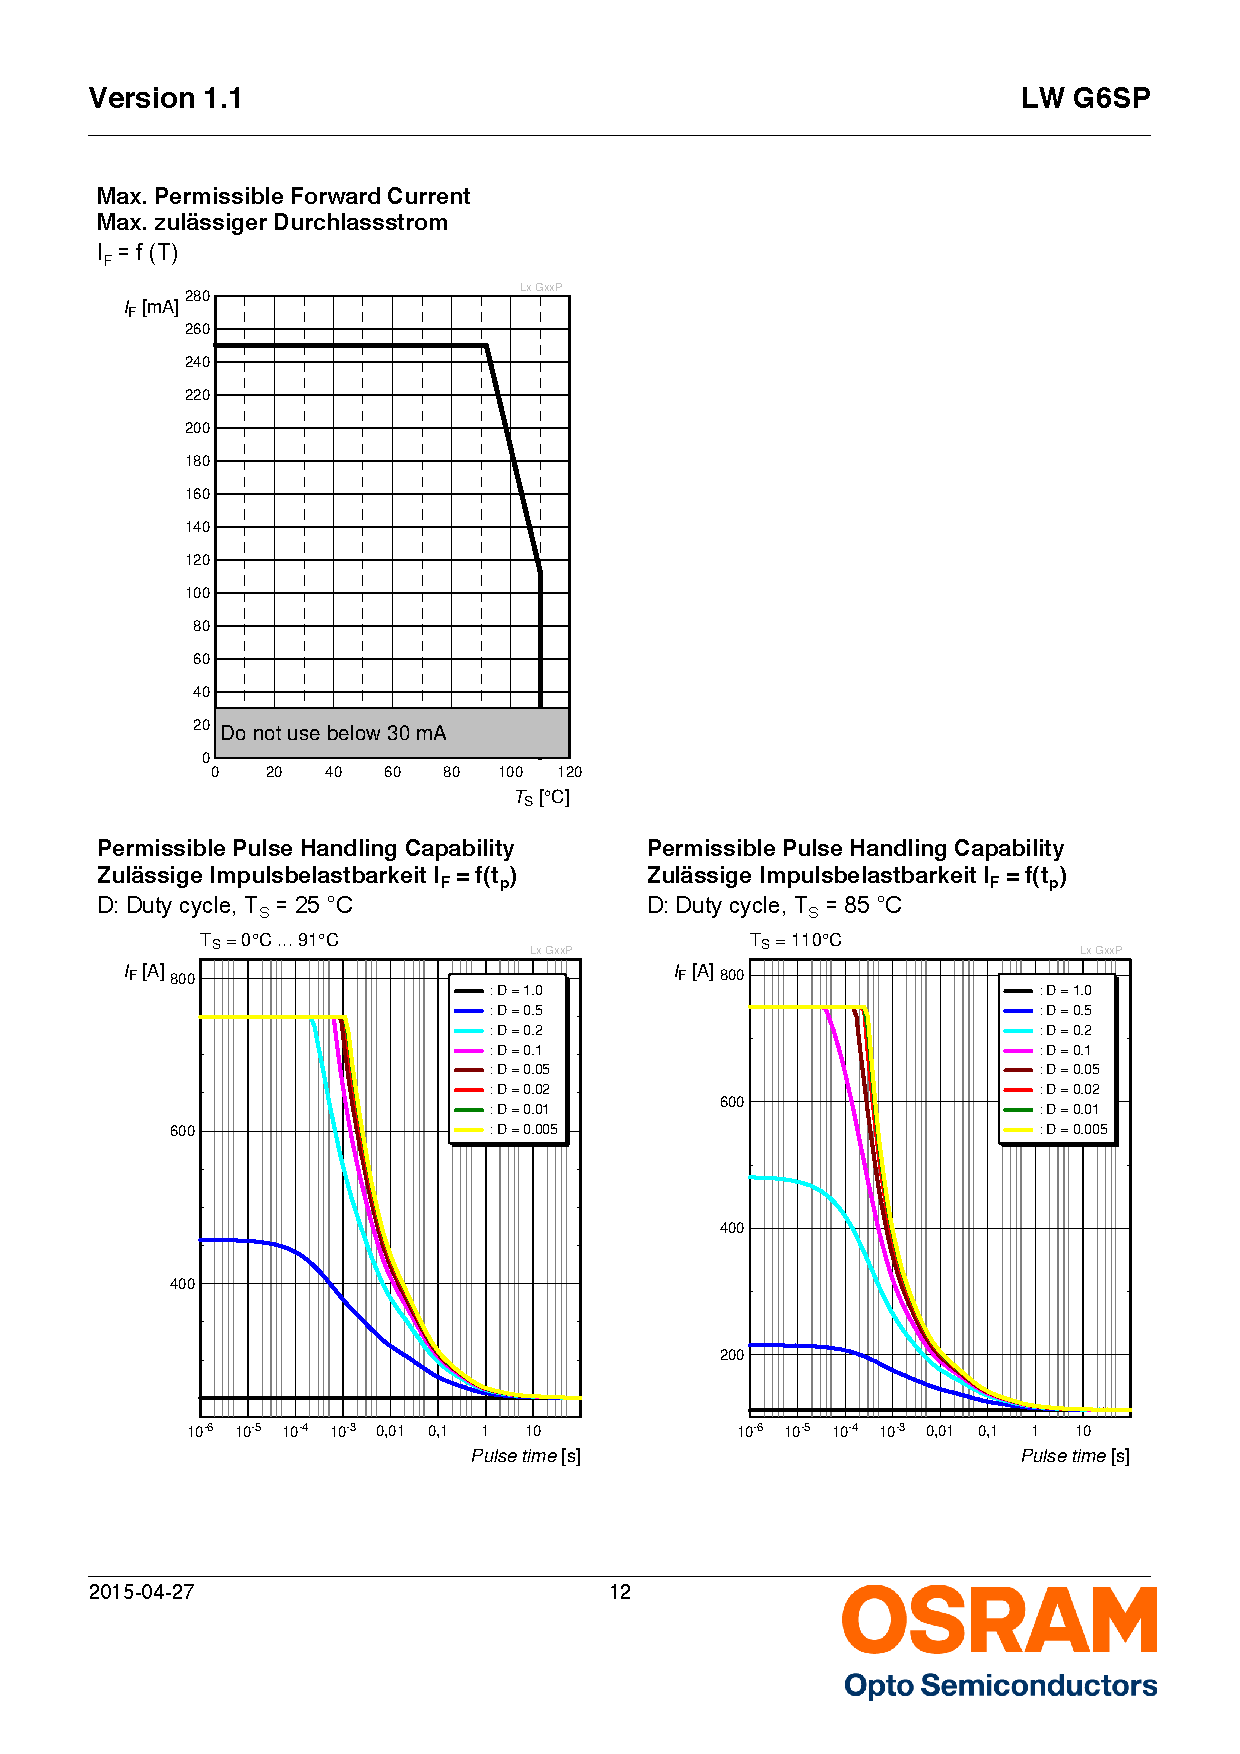
\includegraphics[width=0.3\textheight, trim={2.1cm 4.9cm 10.6cm 15.7cm}, clip]{lw-g6sp-pulse.pdf}
		\legend{Fonte: OSRAM LW-G6SP Datasheet: Advanced Power TOPLED, p. 12}
	\end{figure}
	
	% ---
	\subsection{Fotodiodo}\label{hard-photodiode}
	% ---
	
	O fotodiodo é o componente 
	
	
	% ---
	\subsection{Circuito de Amplificação}\label{hard-opamp}
	% ---
	
	Com intuito de reduzir o ruido da luz ambiente, o circuito passa-faixas amplificador a seguir (\autoref{fig_opampdif}) foi proposto para o projeto.
	
	\begin{figure}[h!]
		\caption{\label{fig_opampdif}Circuito amplificador de diferenças.}
		\centering
		%  trim={<left> <lower> <right> <upper>} 
		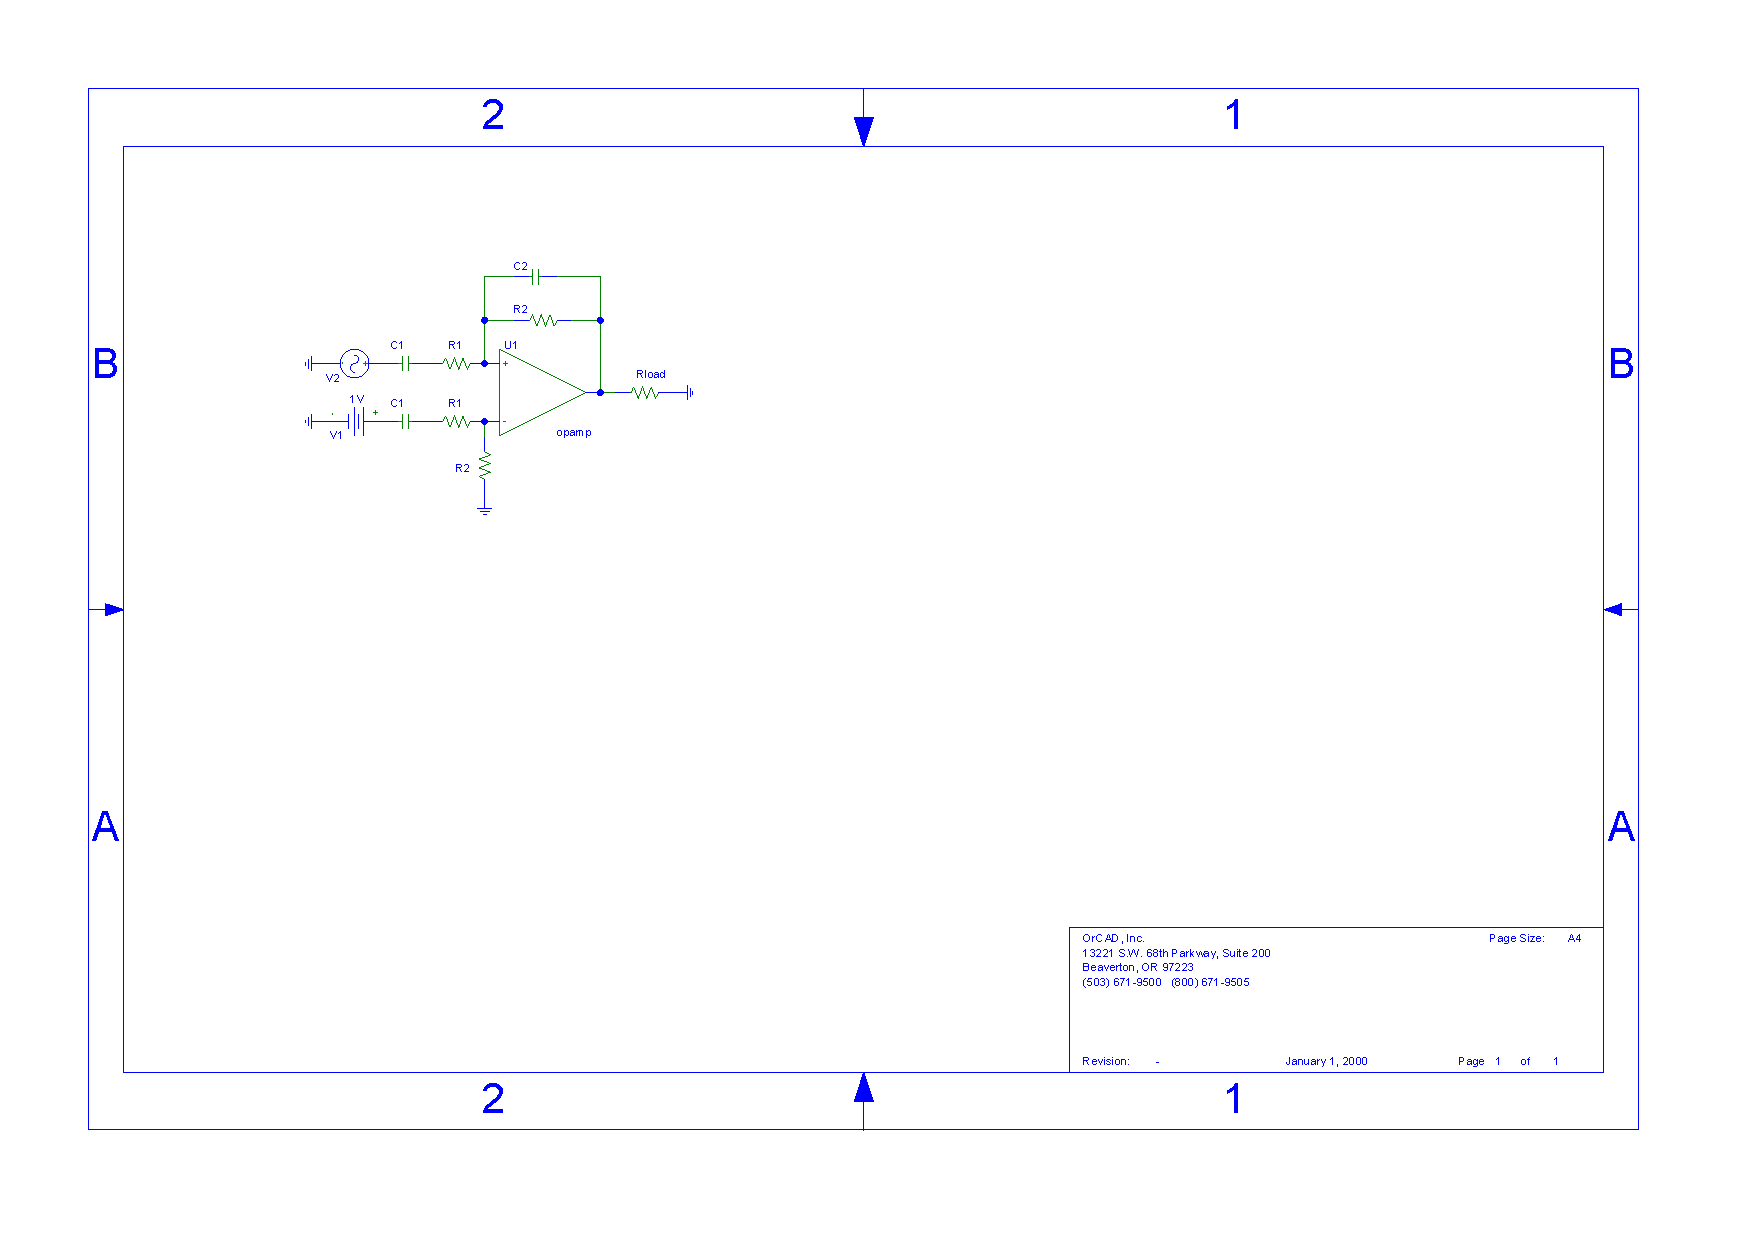
\includegraphics[width=0.6\textwidth, trim={5cm 12.29cm 17.6cm 4.3cm},clip]{opamp-dif2.pdf}
		%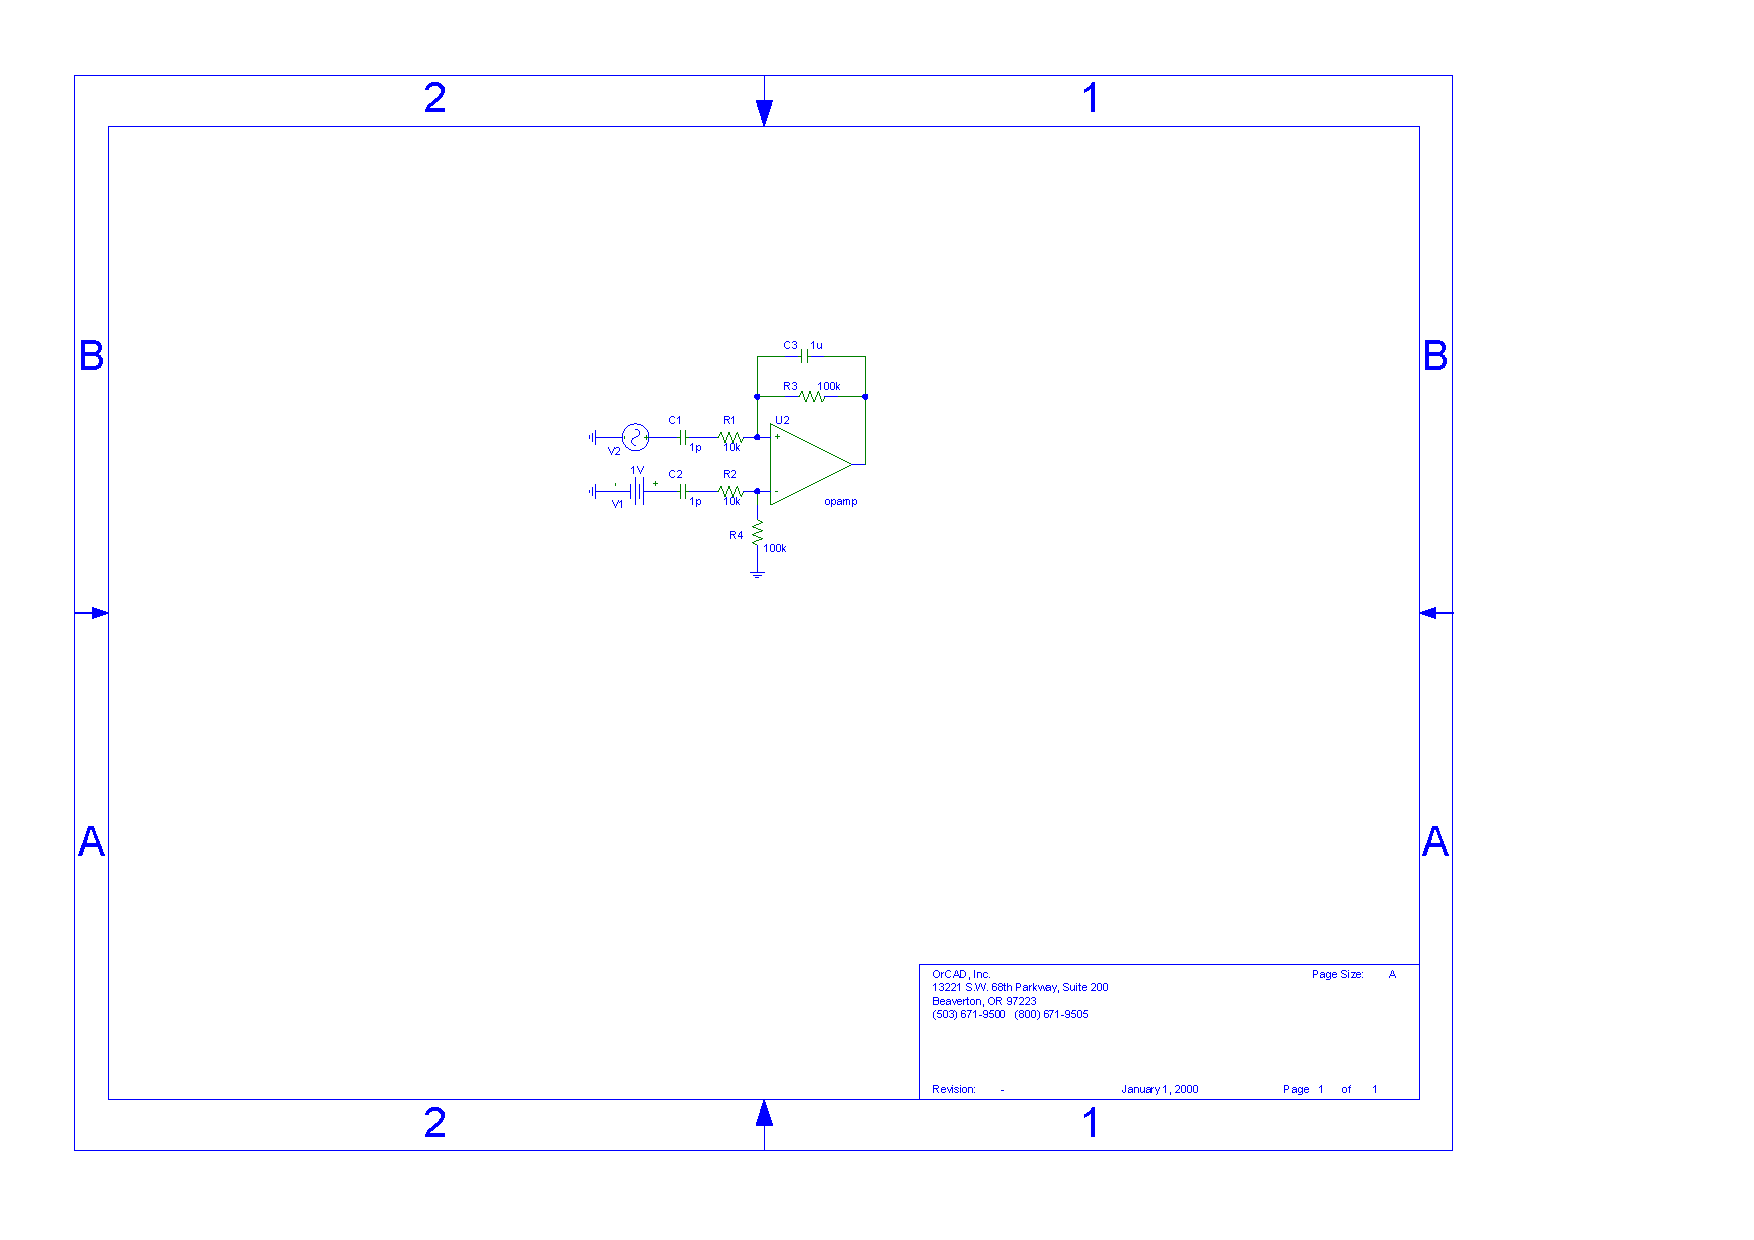
\includegraphics[width=0.5\textwidth, trim={9.5cm 11.2cm 15cm %5.76cm},clip]{opamp-dif.pdf}
		\legend{Fonte: Próprios autores}
	\end{figure}
	
	De acordo com as tabelas \ref{tab_phy1} e \ref{tab_phy2}, o intervalo da frequência do \textit{clock} luminoso é de 200kHz até 120MHz. Deseja-se então  permitir a passagem dessas, limitando as frequências fora desse intervalo. Com o uso do passa baixas e passa altas da figura acima, pode-se realizar essa limitação adequando os resistores e capacitores do circuito.
	
	\begin{figure}[htb]
		\caption{\label{fig_frequenciacentral}Um gráfico em escala logaritmica mostrando a banda de passagem B, a frequência de corte inferior Fl, a frequência de corte superior Fh e a frequência central fo para um circuito passa faixas.}
		\centering
		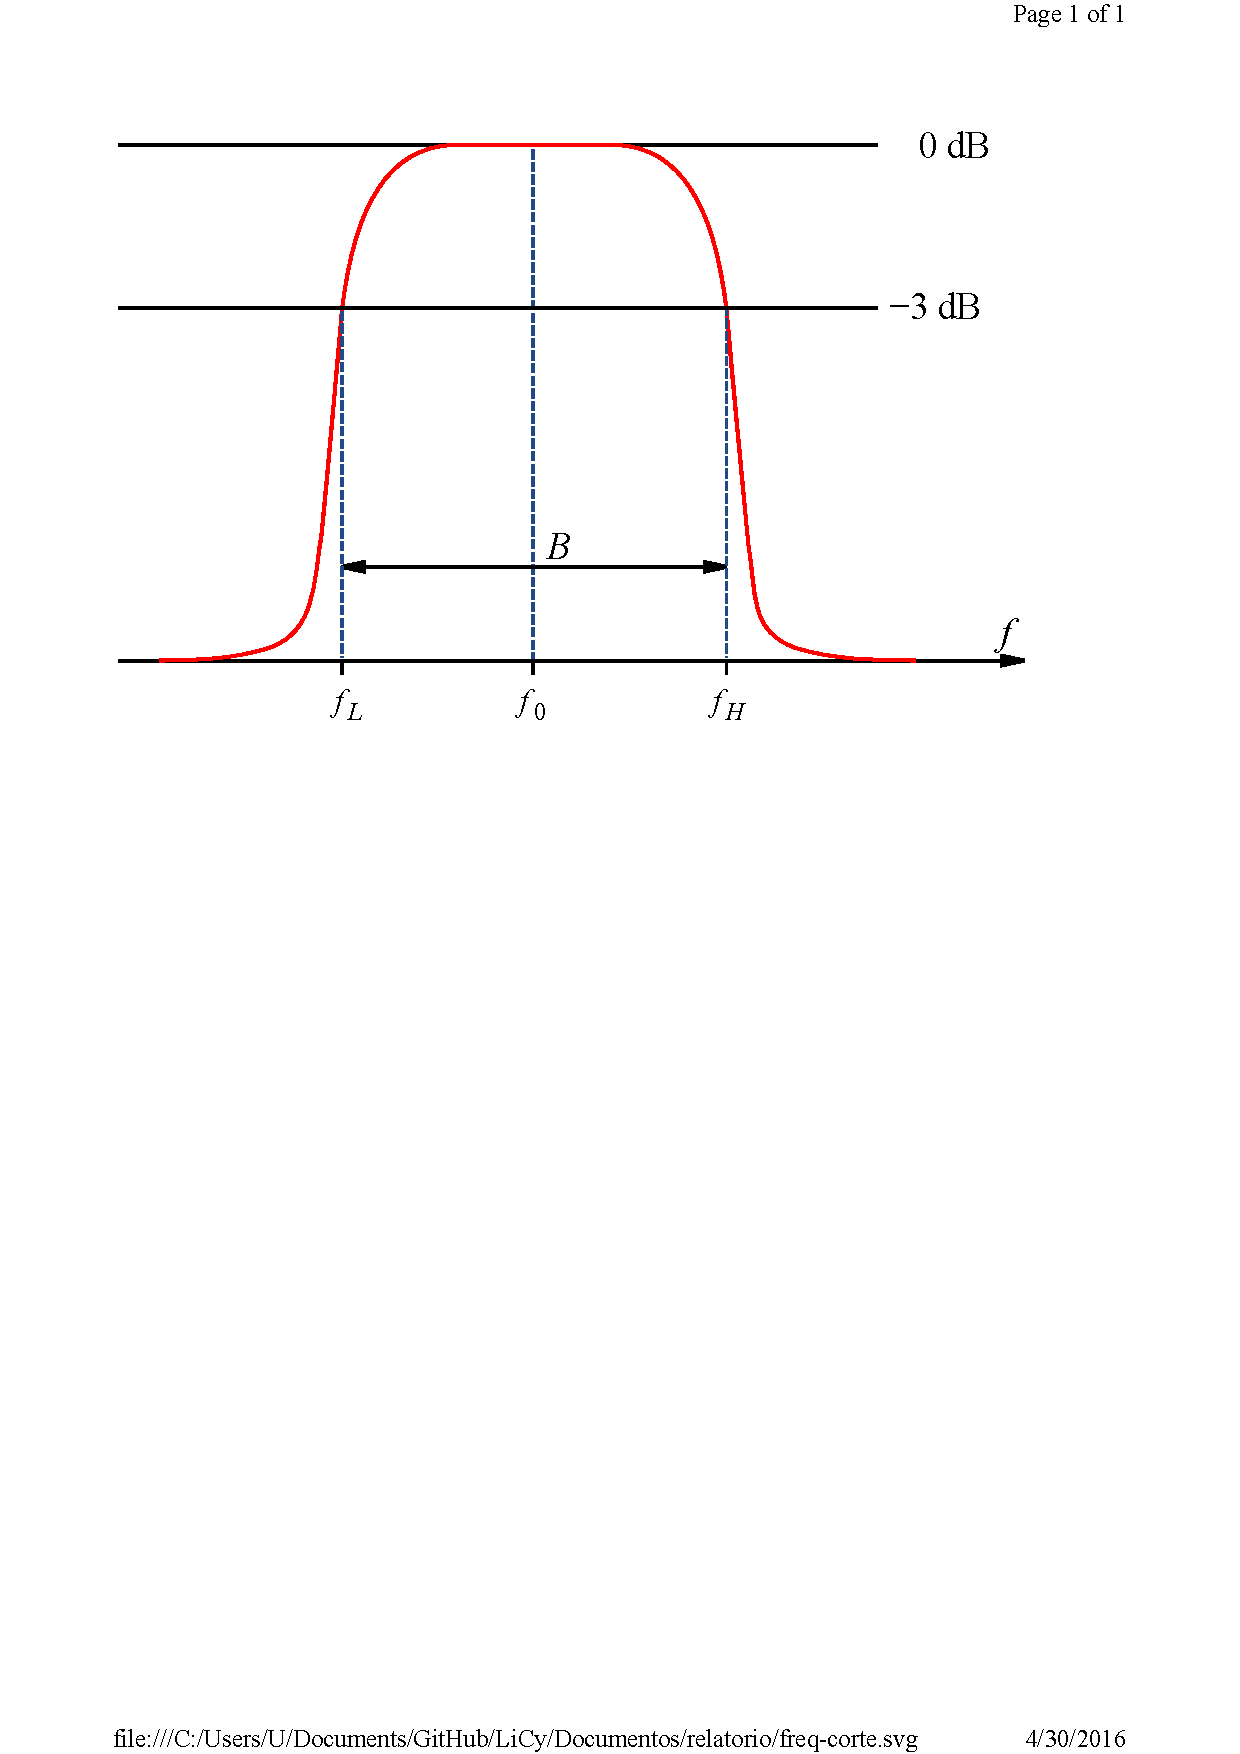
\includegraphics[width=0.5\textwidth, trim={4.5cm 17cm 3.3cm 2cm},clip]{freq-corte.pdf}
		\legend{Fonte: Inductiveload, Wikipedia}
	\end{figure}
	
	Deve-se levar em conta também o ganho do circuito, que é dado pela fórmula:
	
	\begin{equation}
		V_{out} = V_{in} \cdot \frac{R2}{R1}
	\end{equation}
	
	O cálculo da frequência de corte inferior do circuito é dado por: 
	
	\begin{equation} \label{eq:1}
		f_{ci} = \frac{1}{2 \cdot \pi \cdot R1 \cdot C1}
	\end{equation}
	
	No caso da frequência de corte superior, pode-se realizar o cálculo utilizando a fórmula abaixo:
	
	\begin{equation} \label{eq:2}
		f_{ci} = \frac{1}{2 \cdot \pi \cdot R2 \cdot C2}
	\end{equation}
	
	O cálculo da frequência central é feita pela \texttt{média geométrica} das frequências calculadas em \ref{eq:1} and \ref{eq:2} abaixo: 
	
	\begin{equation} \label{eq:3}
		f_{o} = \sqrt{f_{ci} \cdot f_{cs}}
	\end{equation}
	
	A banda de passagem do circuito é calculada pela subtração da frequencia de corte superior pela inferior:
	
	\begin{equation} \label{eq:4}
		BW = f_{cs} - f_{ci}
	\end{equation}
	
	Explicação de porque foi escolhido o circuito com ampop em modo diferencial para o projeto.
	
	% ---
	\section{Software}\label{sec-software}
	% ---
	
	Explica as escolhas feitas no aspecto do software do projeto.
	
	% ---
	\subsection{VHDL}\label{soft-vhdl}
	% ---
	
	Explicação do porquê foi escolhido VHDL
	
	% ---
	\subsubsection{Opções Consideradas}\label{vhdl-options}
	% ---
	
	Explicação de quais foram as opções consideradas.
	
	% ---
	\subsubsection{Tabela Comparativa}\label{vhdl-table}
	% ---
	
	Tabela de opções consideradas.
	
	% ---
	\subsection{Quartus}\label{soft-quartus}
	% ---
	
	Explicação do porquê foi escolhido Quartus
	
	% ---
	\subsubsection{Opções Consideradas}\label{quartus-options}
	% ---

	
	% ---
	\subsubsection{Tabela Comparativa}\label{quartus-table}
	% ---
	
	
	% ---
	\subsection{Android}\label{soft-android}
	% ---
	
	Explicação do porquê foi escolhido Android.
